%% The first command in your LaTeX source must be the \documentclass command.
\documentclass[manuscript,screen,review]{acmart}

%% NOTE that a single column version is required for 
%% submission and peer review. This can be done by changing
%% the \doucmentclass[...]{acmart} in this template to 
%% \documentclass[manuscript,screen,review]{acmart}
%% 
%% To ensure 100% compatibility, please check the white list of
%% approved LaTeX packages to be used with the Master Article Template at
%% https://www.acm.org/publications/taps/whitelist-of-latex-packages 
%% before creating your document. The white list page provides 
%% information on how to submit additional LaTeX packages for 
%% review and adoption.
%% Fonts used in the template cannot be substituted; margin 
%% adjustments are not allowed.
%%
%% \BibTeX command to typeset BibTeX logo in the docs
\AtBeginDocument{%
  \providecommand\BibTeX{{%
    \normalfont B\kern-0.5em{\scshape i\kern-0.25em b}\kern-0.8em\TeX}}}

%% Rights management information.  This information is sent to you
%% when you complete the rights form.  These commands have SAMPLE
%% values in them; it is your responsibility as an author to replace
%% the commands and values with those provided to you when you
%% complete the rights form.
\setcopyright{acmcopyright}
\copyrightyear{2021}
\acmYear{2021}
\acmDOI{10.1145/1122445.1122456}


%%
%% These commands are for a JOURNAL article.
% \acmJournal{POMACS}
% \acmVolume{37}
% \acmNumber{4}
% \acmArticle{111}
% \acmMonth{8}

% *** MACRO FOR MARKING TODO's ***
\usepackage{xcolor}
\newcommand{\todo}[1]{\textcolor{red}{\textbf{\underline{TODO:}} #1}}
\newcommand{\patrick}[1]{\textcolor{blue}{\textbf{\underline{PM:}} #1}}
\newcommand{\ttj}[1]{\textcolor{red}{\textbf{\underline{TTJ:}} #1}}
\newcommand{\diego}[1]{\textcolor{purple}{\textbf{\underline{DM:}} #1}}
\newcommand{\nate}[1]{\textcolor{magenta}{\textbf{\underline{Nate:}} #1}}

% \renewcommand{\todo}[1]{}
% \renewcommand{\patrick}[1]{}
% \renewcommand{\ttj}[1]{}
% \renewcommand{\diego}[1]{}
% \renewcommand{\nate}[1]{}

% \usepackage{todonotes}

\usepackage{color, colortbl}
\definecolor{Gray}{gray}{0.9}
\usepackage{algorithmic}
\usepackage[ruled]{algorithm2e}
\usepackage{graphicx}
\usepackage{multirow}
\usepackage[bottom]{footmisc}
\newcommand{\figref}[1]{Figure~\ref{#1}}



%%
%% The majority of ACM publications use numbered citations and
%% references.  The command \citestyle{authoryear} switches to the
%% "author year" style.
%%
%% If you are preparing content for an event
%% sponsored by ACM SIGGRAPH, you must use the "author year" style of
%% citations and references.
%% Uncommenting
%% the next command will enable that style.
%%\citestyle{acmauthoryear}

%%
%% end of the preamble, start of the body of the document source.
\begin{document}

%%
%% The "title" command has an optional parameter,
%% allowing the author to define a "short title" to be used in page headers.
\title{Online Safety Assurance for Machine Learning Controllers with Real-Time Reachability}

%%
%% The "author" command and its associated commands are used to define
%% the authors and their affiliations.
%% Of note is the shared affiliation of the first two authors, and the
%% "authornote" and "authornotemark" commands
%% used to denote shared contribution to the research.

% \author{Patrick Musau}
% \affiliation{%
%   \institution{Vanderbilt University}
%   \city{Nashville}
%   \state{TN}
%   \country{USA}
%   \postcode{37215}
% }


% \author{Nathaniel Hamilton}
% \affiliation{%
%   \institution{Vanderbilt University}
%   \city{Nashville}
%   \state{TN}
%   \country{USA}
%   \postcode{37215}
% }

% \author{Diego Manzanas Lopez}
% \affiliation{%
%   \institution{Vanderbilt University}
%   \city{Nashville}
%   \state{TN}
%   \country{USA}
%   \postcode{37215}
% }

% \author{Preston Robinette}
% \affiliation{%
%   \institution{Vanderbilt University}
%   \city{Nashville}
%   \state{TN}
%   \country{USA}
%   \postcode{37215}
% }

% \author{Taylor T. Johnson}
% \affiliation{%
%   \institution{Vanderbilt University}
%   \city{Nashville}
%   \state{TN}
%   \country{USA}
%   \postcode{37215}
% }


%%
%% By default, the full list of authors will be used in the page
%% headers. Often, this list is too long, and will overlap
%% other information printed in the page headers. This command allows
%% the author to define a more concise list
%% of authors' names for this purpose.
\renewcommand{\shortauthors}{}

%%
%% The abstract is a short summary of the work to be presented in the
%% article.
\begin{abstract}
  \vspace{-6.5 mm}
Over the last decade, advances in machine learning and sensing technology have paved the way for the belief that the promise of safe, accessible, and convenient autonomous vehicles may be realized in the near future. Despite the prolific competencies of machine learning models for learning the nuances of sensing, actuation, and control, they are notoriously difficult to assure. The challenge here is that some models, such as neural networks, are "black box" in nature, making verification and validation difficult, and sometimes infeasible. Moreover, these models are often tasked with operating in uncertain and dynamic environments where design time assurance may only be partially transferable. Thus, it is critical to monitor these components at runtime. One approach for providing runtime assurance of systems with unverified components is the simplex architecture, where an unverified component is wrapped with a safety controller and a switching logic designed to prevent dangerous behavior. In this paper, we evaluate such an architecture for the safety assurance of a 1/10 scale open source autonomous vehicle platform known as F1/10. Our regime makes use of a real-time reachability algorithm that (a) provides provable guarantees of safety, and (b) is used to detect potentially unsafe scenarios. In our approach, the need to analyze the underlying controller is  abstracted away and instead we   focus on the effects of the controller's decisions on the system's future states. We demonstrate the efficacy of the proposed architecture through experiments conducted both in simulation and on an embedded hardware platform. Furthermore, we present a characterization of the execution times on both platforms, validating the real-time aspects of our approach.
\end{abstract}

%%
%% The code below is generated by the tool at http://dl.acm.org/ccs.cfm.
%% Please copy and paste the code instead of the example below.
%%
% \begin{CCSXML}
% <ccs2012>
%  <concept>
%   <concept_id>10010520.10010553.10010562</concept_id>
%   <concept_desc>Computer systems organization~Embedded systems</concept_desc>
%   <concept_significance>500</concept_significance>
%  </concept>
%  <concept>
%   <concept_id>10010520.10010575.10010755</concept_id>
%   <concept_desc>Computer systems organization~Redundancy</concept_desc>
%   <concept_significance>300</concept_significance>
%  </concept>
%  <concept>
%   <concept_id>10010520.10010553.10010554</concept_id>
%   <concept_desc>Computer systems organization~Robotics</concept_desc>
%   <concept_significance>100</concept_significance>
%  </concept>
%  <concept>
%   <concept_id>10003033.10003083.10003095</concept_id>
%   <concept_desc>Networks~Network reliability</concept_desc>
%   <concept_significance>100</concept_significance>
%  </concept>
% </ccs2012>
% \end{CCSXML}

% \ccsdesc[500]{Computer systems organization~Embedded systems}
% \ccsdesc[300]{Computer systems organization~Redundancy}
% \ccsdesc{Computer systems organization~Robotics}
% \ccsdesc[100]{Networks~Network reliability}


% \keywords{datasets, neural networks, gaze detection, text tagging}



\maketitle

\section{Introduction}
%\todo{Need to change this so that it doesn't include anything from the IROS Paper. Do this last, as this highly depends on the results of other efforts. Part of the story of this paper is that training agents in simulation and then deploying them on real-hardware is a challenging problem. In many cases, the agents do not perform as well as expected. With a set of four controllers that we deploy on real-hardware this can be effectively communicated as an overall story.}


The vision of a "driverless" future has riveted many technology enthusiasts, researchers, and corporations for decades \cite{Badue2019}. The prevailing conviction is that there are relatively few technologies that hold as much promise as autonomous vehicles (AVs) in bringing about safe, accessible, and convenient transportation. Particularly, when the status-quo is considered, far too many individuals still lose their lives to traffic fatalities each year \cite{Rasouli2020}. As Koopman et al. write, "The question is not whether or not autonomous vehicles will be perfect. The question is when [will] we be able to deploy a fleet of fully autonomous driving systems that are actually safe enough to leave the human completely out of the driving loop" \cite{Koopman2017}. 

The two fundamental challenges that are widely regarded as limiting the arrival and widespread adoption of AVs are safety and reliability \cite{Majumdar2017}. Reasoning about safety requires an understanding of the joint dynamics of computers, networks, and physical dynamics in uncertain and variable environments \cite{Yurtsever2019}. Consequently, it is a notoriously difficult problem. To handle the complexities of their environments, many AVs make use of \emph{Machine Learning} (ML) components to decipher the information observed from an ever-evolving configuration of on-board sensors \cite{Yurtsever2019}. Despite the impressive capabilities of these components, there are reservations about using them within safety-critical settings due to their largely opaque nature. Utilizing a "black-box" model within a system that is safety-critical constitutes the highest form of technical debt \cite{Sculley2015} and, as a result, the last several years have witnessed a significant increase in the development of techniques that seek to reason about the safety and robustness of machine learning methods \cite{xiang20118survey}.

% This prevents meaningful statements about their behavior from being made.

%For decades, many technology enthusiasts, researchers, and corporations have had visions of deploying autonomous vehicles on the road~\cite{boudette_2019, Badue2019}. These visions were further emboldened by the success of challenges organized by the Defense Advanced Research Projects Agency (DARPA)~\cite{DARPA_Challenge,driverless_challenges}. The challenges demonstrated the proliferation of autonomous vehicle technology as a vision that could be achieved and spurred the growth of research centers and hundreds of autonomous vehicle companies such as Alphabet's WAYMO, Uber ATG, Argo AI, Aptiv, ZOOX, General Motors' Cruise, Tesla, Aurora, and Intel Corporation's Mobileye \cite{Companies}. While initial projections estimated that autonomous vehicles would be roaming our streets by 2020, today many companies have concluded that the development of robust and safe autonomous vehicles is going to be harder, slower, and more costly than they had originally estimated \cite{driverless_challenges}.

%Among the numerous challenges within this sector, safety is a notoriously difficult problem, and solutions that are both rigorous and practical have yet to be realized \cite{Allen2014}. Autonomous vehicles operate in uncertain, and often unknown environments. Additionally, their perception of this dynamic environment is limited to an ever evolving configuration of on-board sensors \cite{Yurtsever2019}. Within this context, the auspicious results of machine learning methods such as reinforcement learning and deep learning have generated a considerable amount of excitement due to their impressive capabilities in dealing with complex data. However, there are reservations about using them within safety-critical settings due to the difficulty of interpreting the inner workings of these models, which prevents any meaningful statements about their behavior from being made. 

%Typically, in simplex architectures, the switching logic is primarily designed either from a control theoretic perspective through the solution of linear matrix inequalities (LMI) \cite{SetoCaseStudy2000}, or using a formal analysis hybrid-systems reachability technique \cite{Bak2009Simplex}.



Unfortunately, while numerous works have been proposed in the past few years for the formal analysis of machine learning methods, the vast majority of these efforts have not been able to scale to the complexity found in real world applications, where models such as neural networks may be characterized by millions or even billions of parameters \cite{SimonyanVeryDeep}. Thus, designing solutions that are both practical and rigorous is extremely challenging. One approach that has enabled the assurance of systems with unverified components is the \textit{simplex architecture}. In this framework, an unverified component is wrapped with a safety controller and switching logic designed to transfer control to the safety controller in certain situations \cite{Bak2014}. The key challenge in this regime is to design a switching logic that allows the dynamic capabilities of the unverified, complex controller to be exploited without compromising safety. In this paper, we extend a real-time reachability algorithm \cite{Bak2014,Johnson2016} to design a simplex architecture for a $1/10$ scale autonomous racing car called the F1/10 platform. %\diego{I see the point of this paragraph, but it could be confusing. Simplex is an architecture used to switch controllers, it is not a formal analysis of NNs. I will add maybe one more sentence clarifying that there are other ways of dealing with nn controllers such as simplex, or other runtime monitoring/assurance methods that reason about the system while operating, instead of reasoning about the controller at design/offline time. You mention that this work is runtime assurance in the next paragraph, but if I did not know what you are trying to do, I'd be confused}

 To put our work into context, this work falls within the \textit{runtime verification} or \textit{runtime assurance} realm. Our aim is to construct an architecture that allows us to ensure that an autonomous vehicle, controlled using machine learning strategies, never enters unsafe states as it navigates an environment. Specifically, the set of control strategies presented herein were synthesized using reinforcement learning and imitation learning, which have generated a considerable amount of excitement in recent years \cite{bojarski2016end,lillicrap2015continuous}. Our approach abstracts away the need to analyze the underlying nature of these controllers and instead observes the influence of control actions on the system behavior at runtime. %This makes it particularly applicable to machine learning systems. 
%\todo{I can replace this figure of the F1Tenth with another one. This one has already been submitted to another conference.}
%\begin{figure}%[htp!]
%  \centering
%    % \hspace*{-8mm}  
%    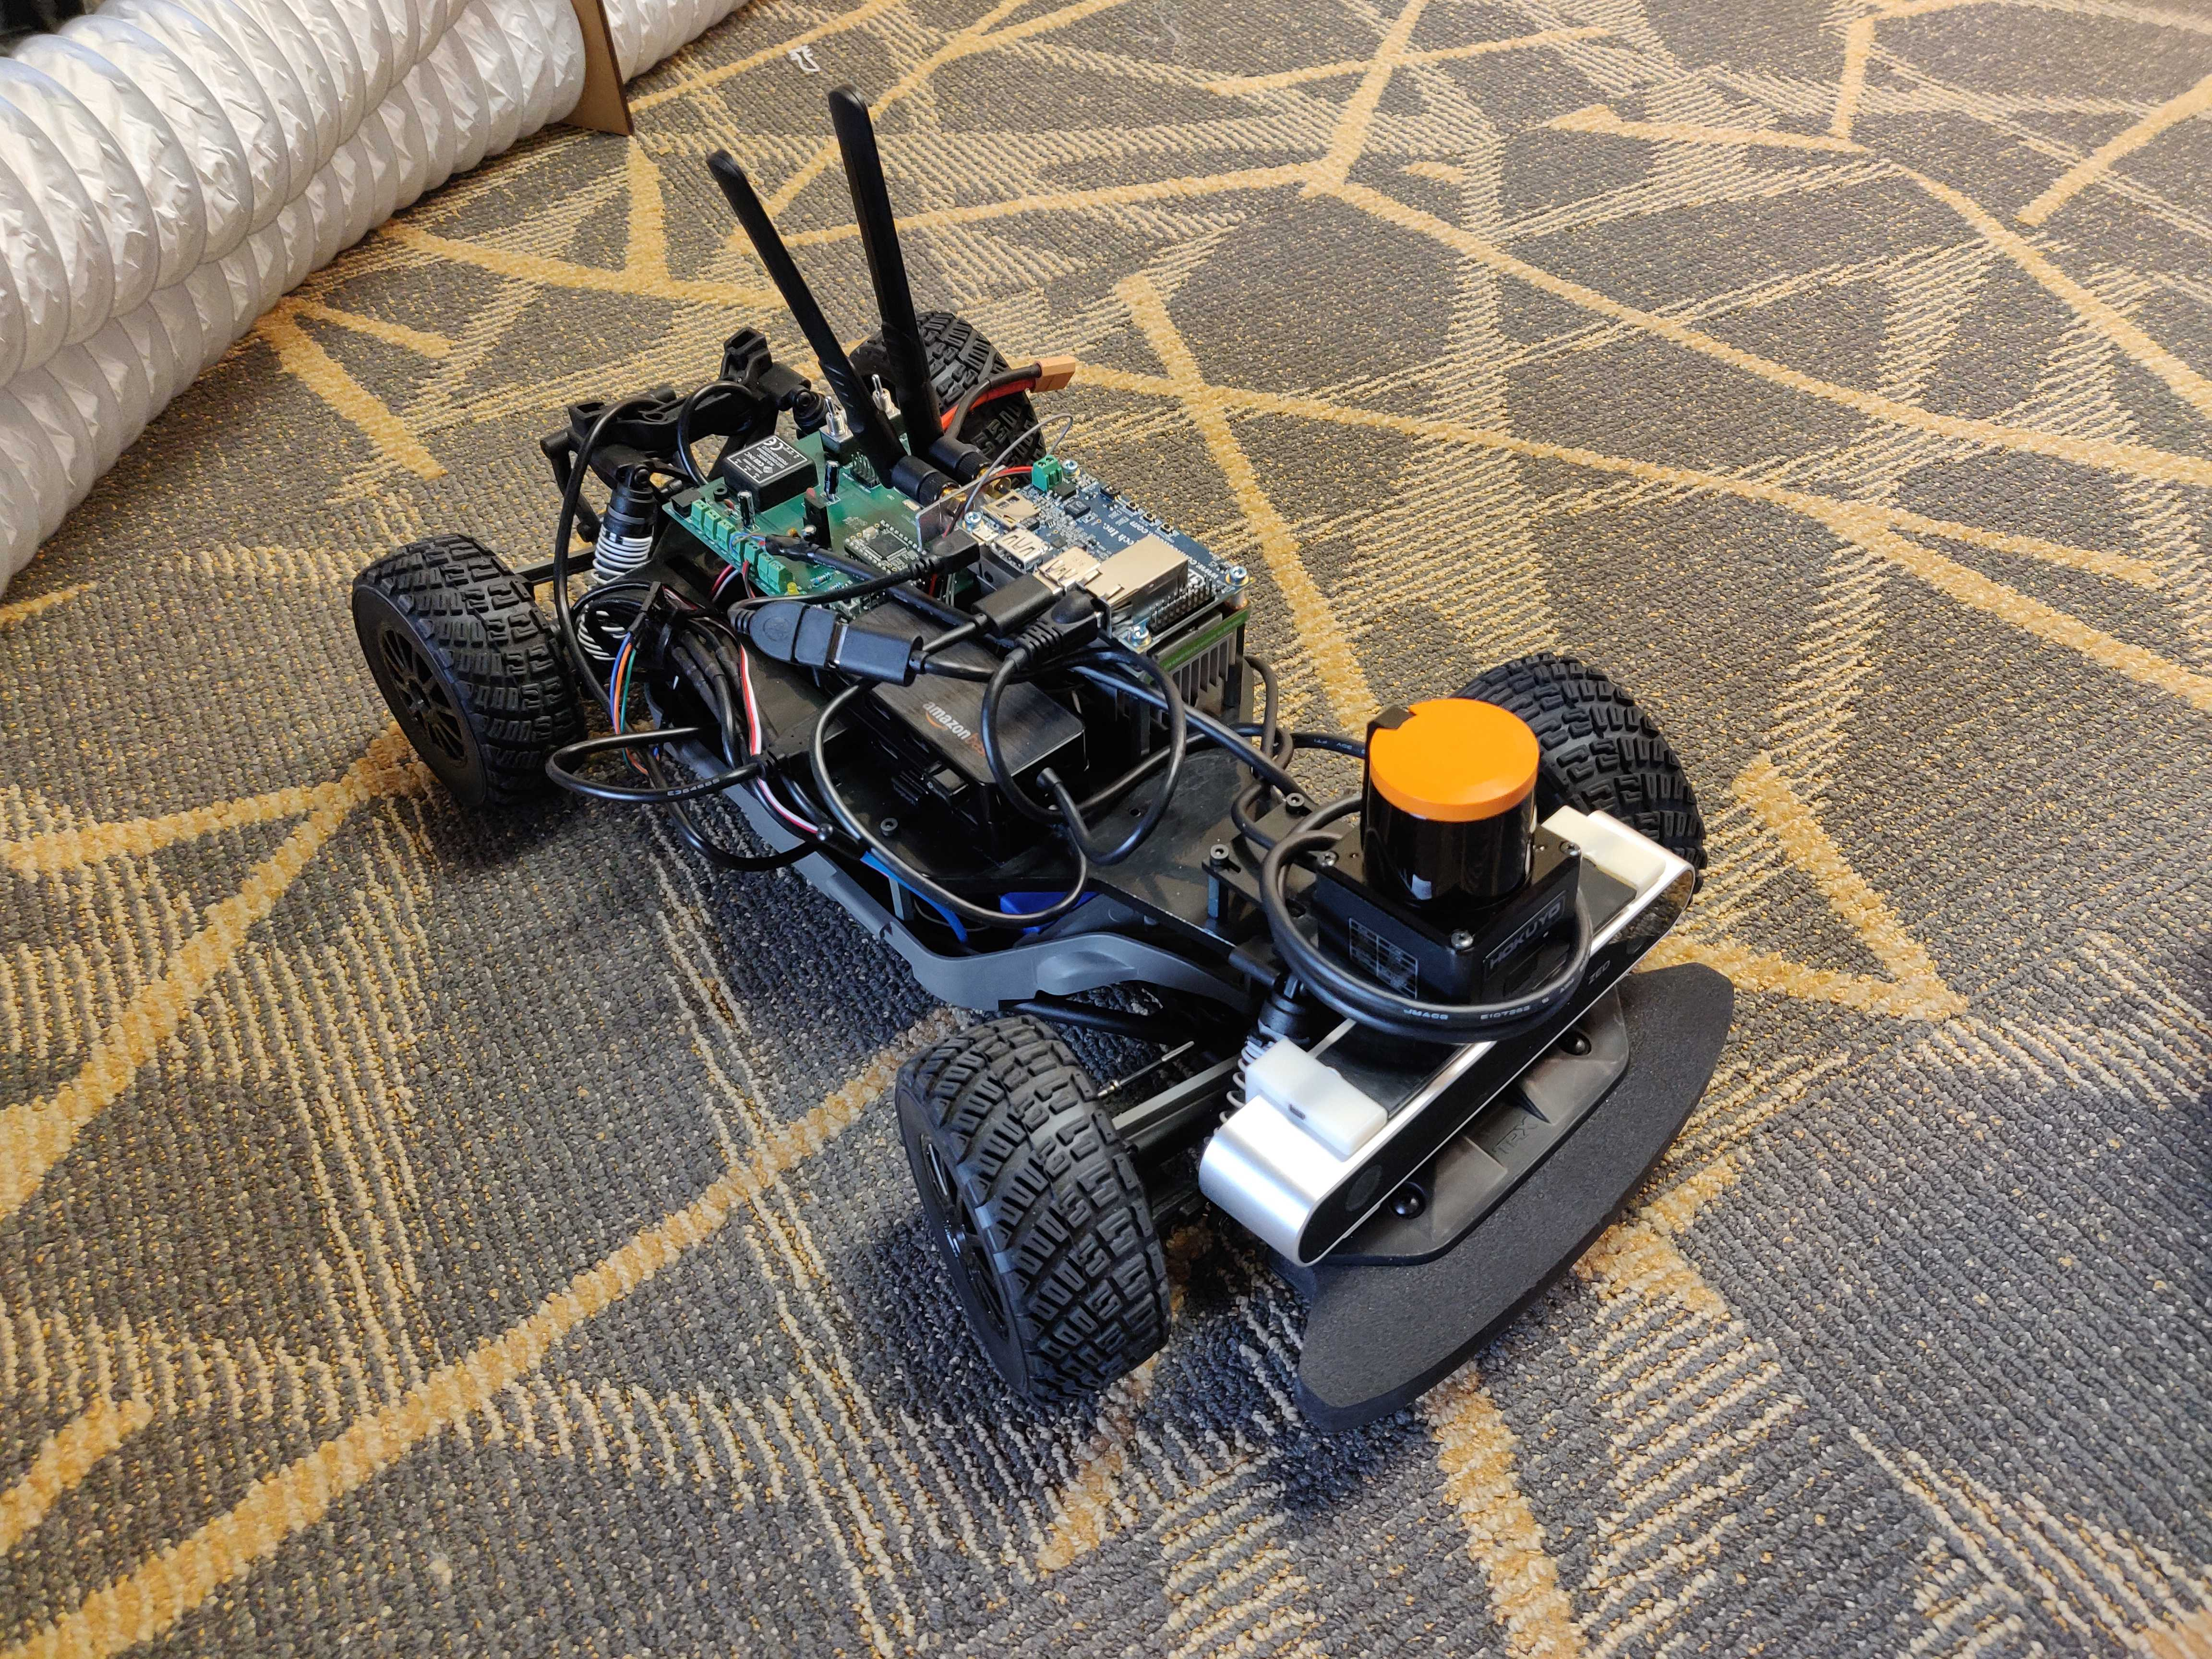
\includegraphics[width=0.5\linewidth]{f1tenth.jpg}
%   \caption{Visualization of our experimental F1/10 hardware platform. This platform is a one-tenth scale RC car that has been altered to entertain autonomous control inputs as well as support a sensor and compute architecture for autonomous decision making. \cite{okelly2020}. }
%  \label{fig:f1tenth_hardware}
%\end{figure}

To perform the verification, we first identify a dynamical model of the car and assume that the car operates within an \textit{a priori} known environment. Next, we synthesize controllers using data collected from a series of experiments with the F1/10 vehicle, as well as through the execution of a series of reinforcement learning training campaigns. Using the obtained controllers, we aim to verify that the car does not crash into static obstacles within its environment as well as the environment boundaries. To do this, we extend a real-time reachability algorithm proposed by Bak et al. \cite{Bak2014,Johnson2016} to compute the set of reachable states for a finite time-horizon and check for potential collisions. This safety checking forms the basis of the switching scheme in our simplex architecture, and we evaluate the merits of this approach both in simulation and on the F1/10 hardware platform using a variety of controllers, number of obstacles, and runtime configurations.

In summary, the contributions of this paper are: \raggedbottom
\begin{itemize}%
    \item We extend a previous simplex control architecture that makes use of a real-time reachability algorithm based on mixed face-lifting to an autonomous race car both in simulation and on an embedded platform.
    \item We modify the real-time reachability algorithm presented in \cite{Bak2014} to handle static obstacles in a sound and real-time manner.
    \item We present a regime that abstracts away the need to analyze opaque machine learning models and instead observes the influence of their decisions on the system during operation.
    %\item We train two learning-enabled, or "black-box", controllers.
    \item We demonstrate success using the simplex architecture to safely navigate through obstacles, with which the trained controllers have no prior experience.
    \item We evaluate the safety of machine learning components transferred to real-world hardware without additional training.
    
\end{itemize}%



\section{Background: The Simplex Architecture and Real-Time Reachability}
\subsection{Simplex Architecture}

%As modern autonomous systems grow in complexity, so do the challenges in assessing their reliability and correctness \cite{Bak2009Simplex}. Moreover, any arguments about the reliability and safety of the system rely on assertions about the individual components that make it up \cite{Bak2014}. However, in recent years, with the growth of increasingly autonomous systems \cite{Jha2020}, individual components may be designed using machine learning methods, such as neural networks, that are opaque to traditional formal analysis. Despite the recent years' surge in the development of formal analysis techniques for these types of models \cite{Liu2019,xiang20118survey}, most techniques are incapable of dealing with the scale of models deployed in state-of-the-art systems.

One paradigm for dealing with untrustworthy components is the \emph{simplex architecture} \cite{RiveraAnArchitectural1996}. In the simplex architecture, the unverified component, or \emph{complex controller}, is wrapped with a \emph{safety controller} and a switching logic used to ensure safety~\cite{Bak2014}. A useful analogy for this architecture is a driving instructor's car with two steering wheels and two sets of brakes. As long as the instructor is capable of intervening in dangerous situations, the capricious student is allowed to drive. Typically, the complex controller has better performance with respect to the design metrics, whereas the safety controller is designed with simplicity and verifiability in mind. Thus, by using this architecture, one can utilize the complex controller while still maintaining the formal guarantees of the safety controller. The key challenge when designing a system with the simplex architecture is properly designing the switching logic \cite{Johnson2016}. One must be able to clearly delineate safe states from unsafe states. 

Typically, in simplex architectures, the switching logic is primarily designed either from a control theoretic perspective through the solution of linear matrix inequalities (LMI) \cite{SetoCaseStudy2000}, or using a formal analysis hybrid-systems reachability technique \cite{Bak2009Simplex}. In this paper, our simplex design necessitates computing the set of reachable states online through the use of a real-time reachability algorithm for short time horizons.


\subsection{Real-Time Reachability}

Reachability algorithms have traditionally been executed offline and are typically computationally intensive endeavors \cite{Chen2013,AlthoffCORA2015,manzanas2019arch_ainncs}. However, in \cite{Bak2014,Johnson2016}, Bak et al., and Johnson et al. presented a reachability algorithm, based on the influential mixed face-lifting algorithm \cite{dang2000}, capable of running in real-time on embedded processors. The algorithm is implemented as a standalone C-package that does not rely on sophisticated (non-portable) libraries, recursion, or dynamic data structures and is amenable to the anytime computation model in the real-time scheduling literature \cite{Liu1991}. In this regime, each task produces a partial result that is improved upon as more computation time is added \cite{Johnson2016}. 

The controllers used in our experiments are designed to sample sensor data and compute control actions at fixed time intervals as typically done in the control community \cite{Dai2020}. During each control period, we take the corresponding control action and compute the reachable set of states into the future as defined by the current state and a specified finite-time horizon. An example of this computation is shown in \figref{fig:reachset}. We assume a fixed control action throughout the reachable set computation. Based on the obtained reachable set, we determine if the system will collide with objects in its environment and, if necessary, switch to a safety controller optimized for obstacle avoidance. If the system falls back to using a safety controller, we only allow a switch back to the complex controller if the complex controller has demonstrated safe behavior for a fixed number of control periods\footnote{In our experiments we allowed a switch back to the safety controller after 25 control periods. This corresponds to 1.25 seconds using a $20\ Hz$ control period.}. This prevents arbitrary switching and incorporates a sense of hysteresis into our control strategy. Additionally, by not switching back until consistently safe behavior has been demonstrated, we enforce a notion of dwell time, which reduces instabilities caused by switching too frequently. %Our approach has successfully been deployed to ensure safety both in simulation and on the F1/10 hardware platform.


\begin{figure}[htpb]%[!htb]
  \centering
    % \hspace*{-8mm}  
    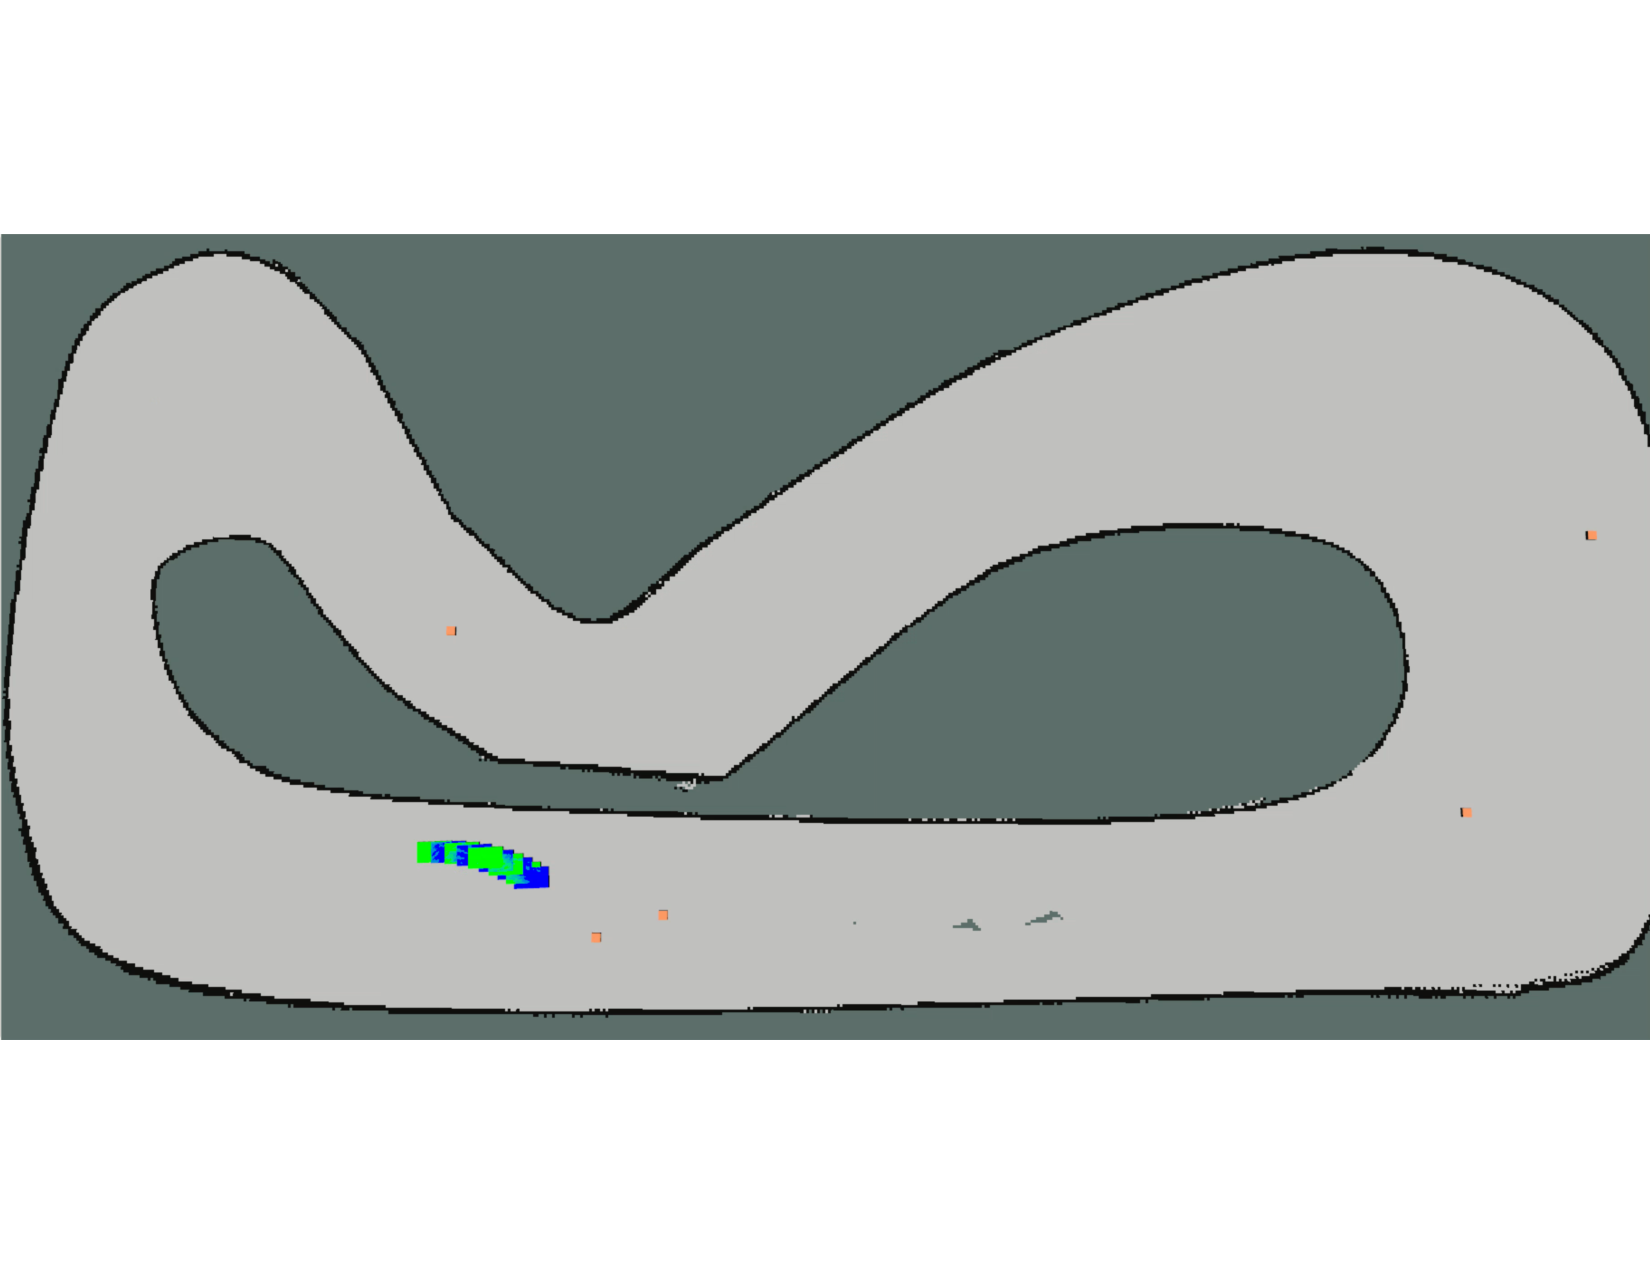
\includegraphics[width=0.75\linewidth]{figures/viz_option_two.pdf}
   \caption{Visualization of the set of reachable states using the current control action. For illustration purposes, we display only a subset of the hyper-rectangles making up the reachable set. This example corresponds to a safe scenario, as there is no intersection with obstacles or the the racetrack walls. The orange squares represent the location of cones and their corresponding bounding box.}
  \label{fig:reachset}
\end{figure}



\section{Experimental Overview}

To build and assure the safety of our system at runtime, we perform the following steps. First, we construct a mathematical model of the F1/10 car's physical dynamics using system identification techniques. We then deploy one of our machine learning (ML) controllers into the control architecture. These controllers are: (1) Imitation Learning controllers trained to mimic driving behavior using data collected from a series of experimental runs of driving with a baseline controller and (2) Reinforcement Learning controllers (RLc), i.e. a control policy trained using an RL algorithm. The controllers use sensor information to determine the desired steering angle for the vehicle. At runtime, the mathematical model obtained through system identification is used within the reachability algorithm to reason about safety of the control actions selected by the ML controllers. The simplex architecture provides the framework for ensuring safe operation of the F1/10.


%At runtime, using the mathematical model that we obtained through system identification and our real-time reachability algorithm, we compute the reachable set of states from the current state and the control input given by our controller, for a specified reach time. During the construction of the reachable set, we perform safety checking in order to gauge whether the reachable set of states intersects with known obstacles or the walls defining the track environment. Lastly, based on the results of the safety checking, we design a simplex strategy to maintain safe operation of the F1/10 model. 

\subsection{The F1/10 Autonomous Platform}

The F1/10 platform proposed by Matthew O'Kelly et al. in \cite{F1102019} was originally designed to emulate the hardware and software capabilities of full scale autonomous vehicles. The platform is equipped with a standard suite of sensors such as stereo cameras, LiDAR (light detection and ranging), and inertial measurement units (IMU). The platform uses an NVIDIA Jetson TX2 as its compute platform, and its software stack is built on the \emph{Robot Operating System} (ROS)\footnote{It is worth noting that ROS is not an operating system in the traditional sense but rather a meta-operating system that primarily provides the message passing interface for various components within robot software development \cite{Huang2014}.} \cite{ROS}. The result is a platform that allows researchers to conduct real-world experiments that investigate planning, networking, and intelligent control on a relatively low-cost, open-source test-bed \cite{F1102019}. Additionally, in order to promote rapid prototyping and consider research questions around closing the simulation to reality gap\cite{Muratore2019}, Varundev Suresh et al. designed a Gazebo-based simulation environment \cite{Gazebo} that includes a realistic model of the F1/10 platform and its sensor stack \cite{varundev_ros_19}. We utilize this simulation environment for a number of experiments and training our controllers.

%\todo{For this version of the paper, we are going to evaluate a whole set of controllers. I can present some of the results from the IL vs RL paper not in the exact same way but just their different efficacies and reachability results}

\subsection{Vehicle Dynamics Model and System Identification}


\begin{figure}[htbp]%
  \centering
    % \hspace*{-8mm}  
    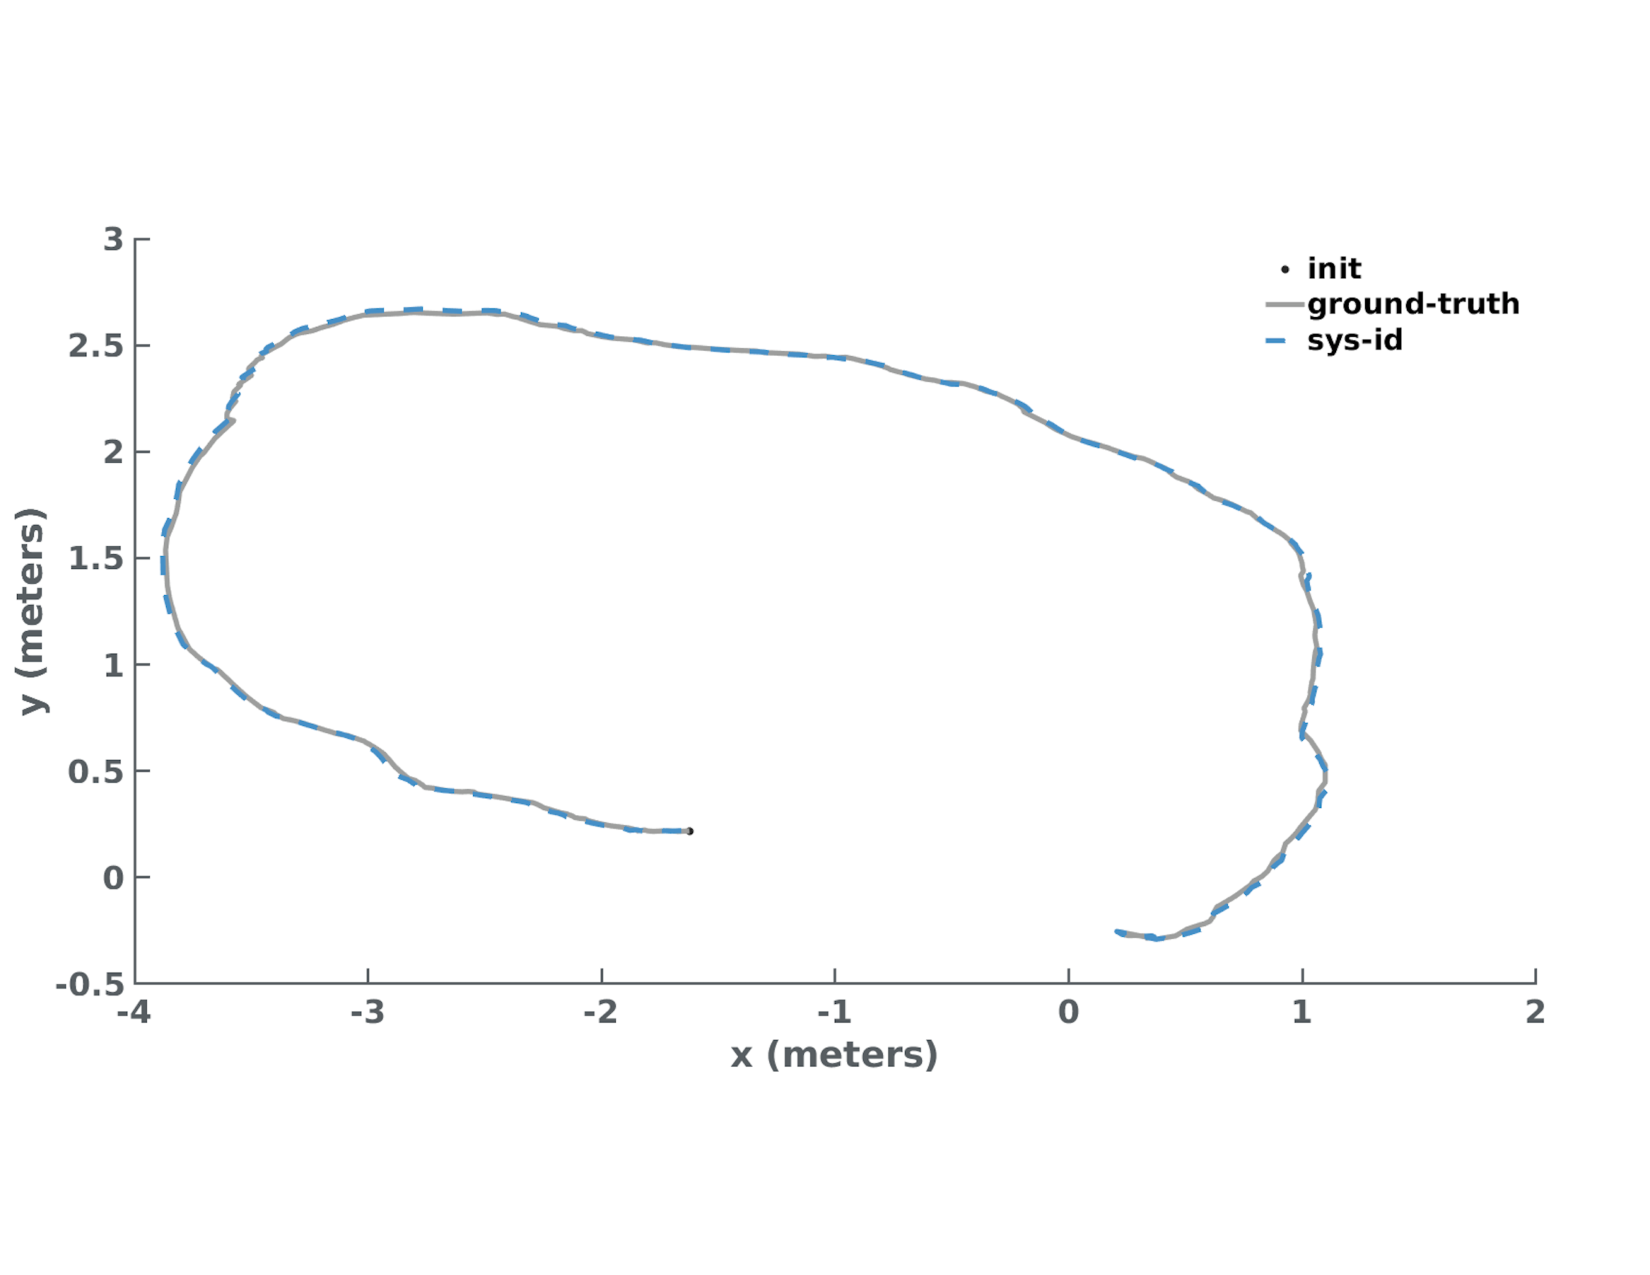
\includegraphics[width=0.70\linewidth]{figures/sys_id2_2.pdf}
  \caption{Vehicle Position (map frame). Model validation for the F1/10 Hardware Model using data collected from a manual set of experimental runs. \emph{Init} corresponds to the starting position of the vehicle in the considered experiment.}
  \label{fig:validation}
\end{figure}%


The physical dynamics of the F1/10 vehicle are modeled using a kinematic bicycle model \cite{Rajamani2012}, which is described by a set of four-dimensional nonlinear ordinary differential equations (ODEs). The kinematic bicycle model is characterized by relatively few parameters and tracks reasonably well at low speeds.\footnote{ The kinematic bicycle model typically tracks well under $5 m/s$ \cite{ivanov2020case}} The model has four states: Euclidean positions $x$ and $y$, linear velocity $v$, and heading $\theta$. The dynamics are given by the following ODEs: 
\begin{align*}
    \Dot{x} & = v\cos(\theta +\beta)\\
    \Dot{y} & = v\sin(\theta + \beta)\\
    \Dot{v} & = -c_av +c_ac_m(u-c_h)\\
    \Dot{\theta} & = \frac{v\cos(\beta)}{l_f+l_r}\tan(\delta)\\
    \beta &= \tan^{-1}\Big(\frac{l_r\tan(\delta)}{l_f+l_r}\Big),
\end{align*}




\noindent where $v$ is the car's linear velocity, $\theta$ is the car's orientation, $\beta$ is the car's slip angle, $x$ and $y$ are the car's position, $u$ is the throttle input, $\delta$ is the steering input, $c_a$ is an acceleration constant, $c_m$ is a motor constant, $c_h$ is a hysteresis constant, and $l_f$ and $l_r$ are the distances from the car's center of mass to the front and rear respectively \cite{ivanov2020case}. For simplicity, since the slip angle is fairly small at low speeds, we assume that $\beta = 0$.
Using MATLAB's Grey-Box System Identification toolbox, we obtained the following parameters for the simulation model: $c_a = 1.9569$, $c_m = 0.0342$, $c_h = -37.1967$, $l_f =0.225$, $l_r = 0.225$. The model was validated using a series of experiments %\footnote{The code used for system identification and model validation can be found at: \url{https://github.com/pmusau17/Platooning-F1Tenth/tree/master/src/race/sys_id}}
with an average \emph{Mean Squared Error} (MSE) of $0.003$. A sample experimental simulation is shown in \figref{fig:validation}. For the hardware platform, we obtained the following parameters: $c_a = 2.9820$, $c_m = 0.0037$, $c_h = -222.1874$, $l_f =0.225$, $l_r = 0.225$, with a validation MSE of $6.75 \times 10^{-4}$.







% \begin{figure}[htbp]%
%   \centering
%     % \hspace*{-8mm}  
%     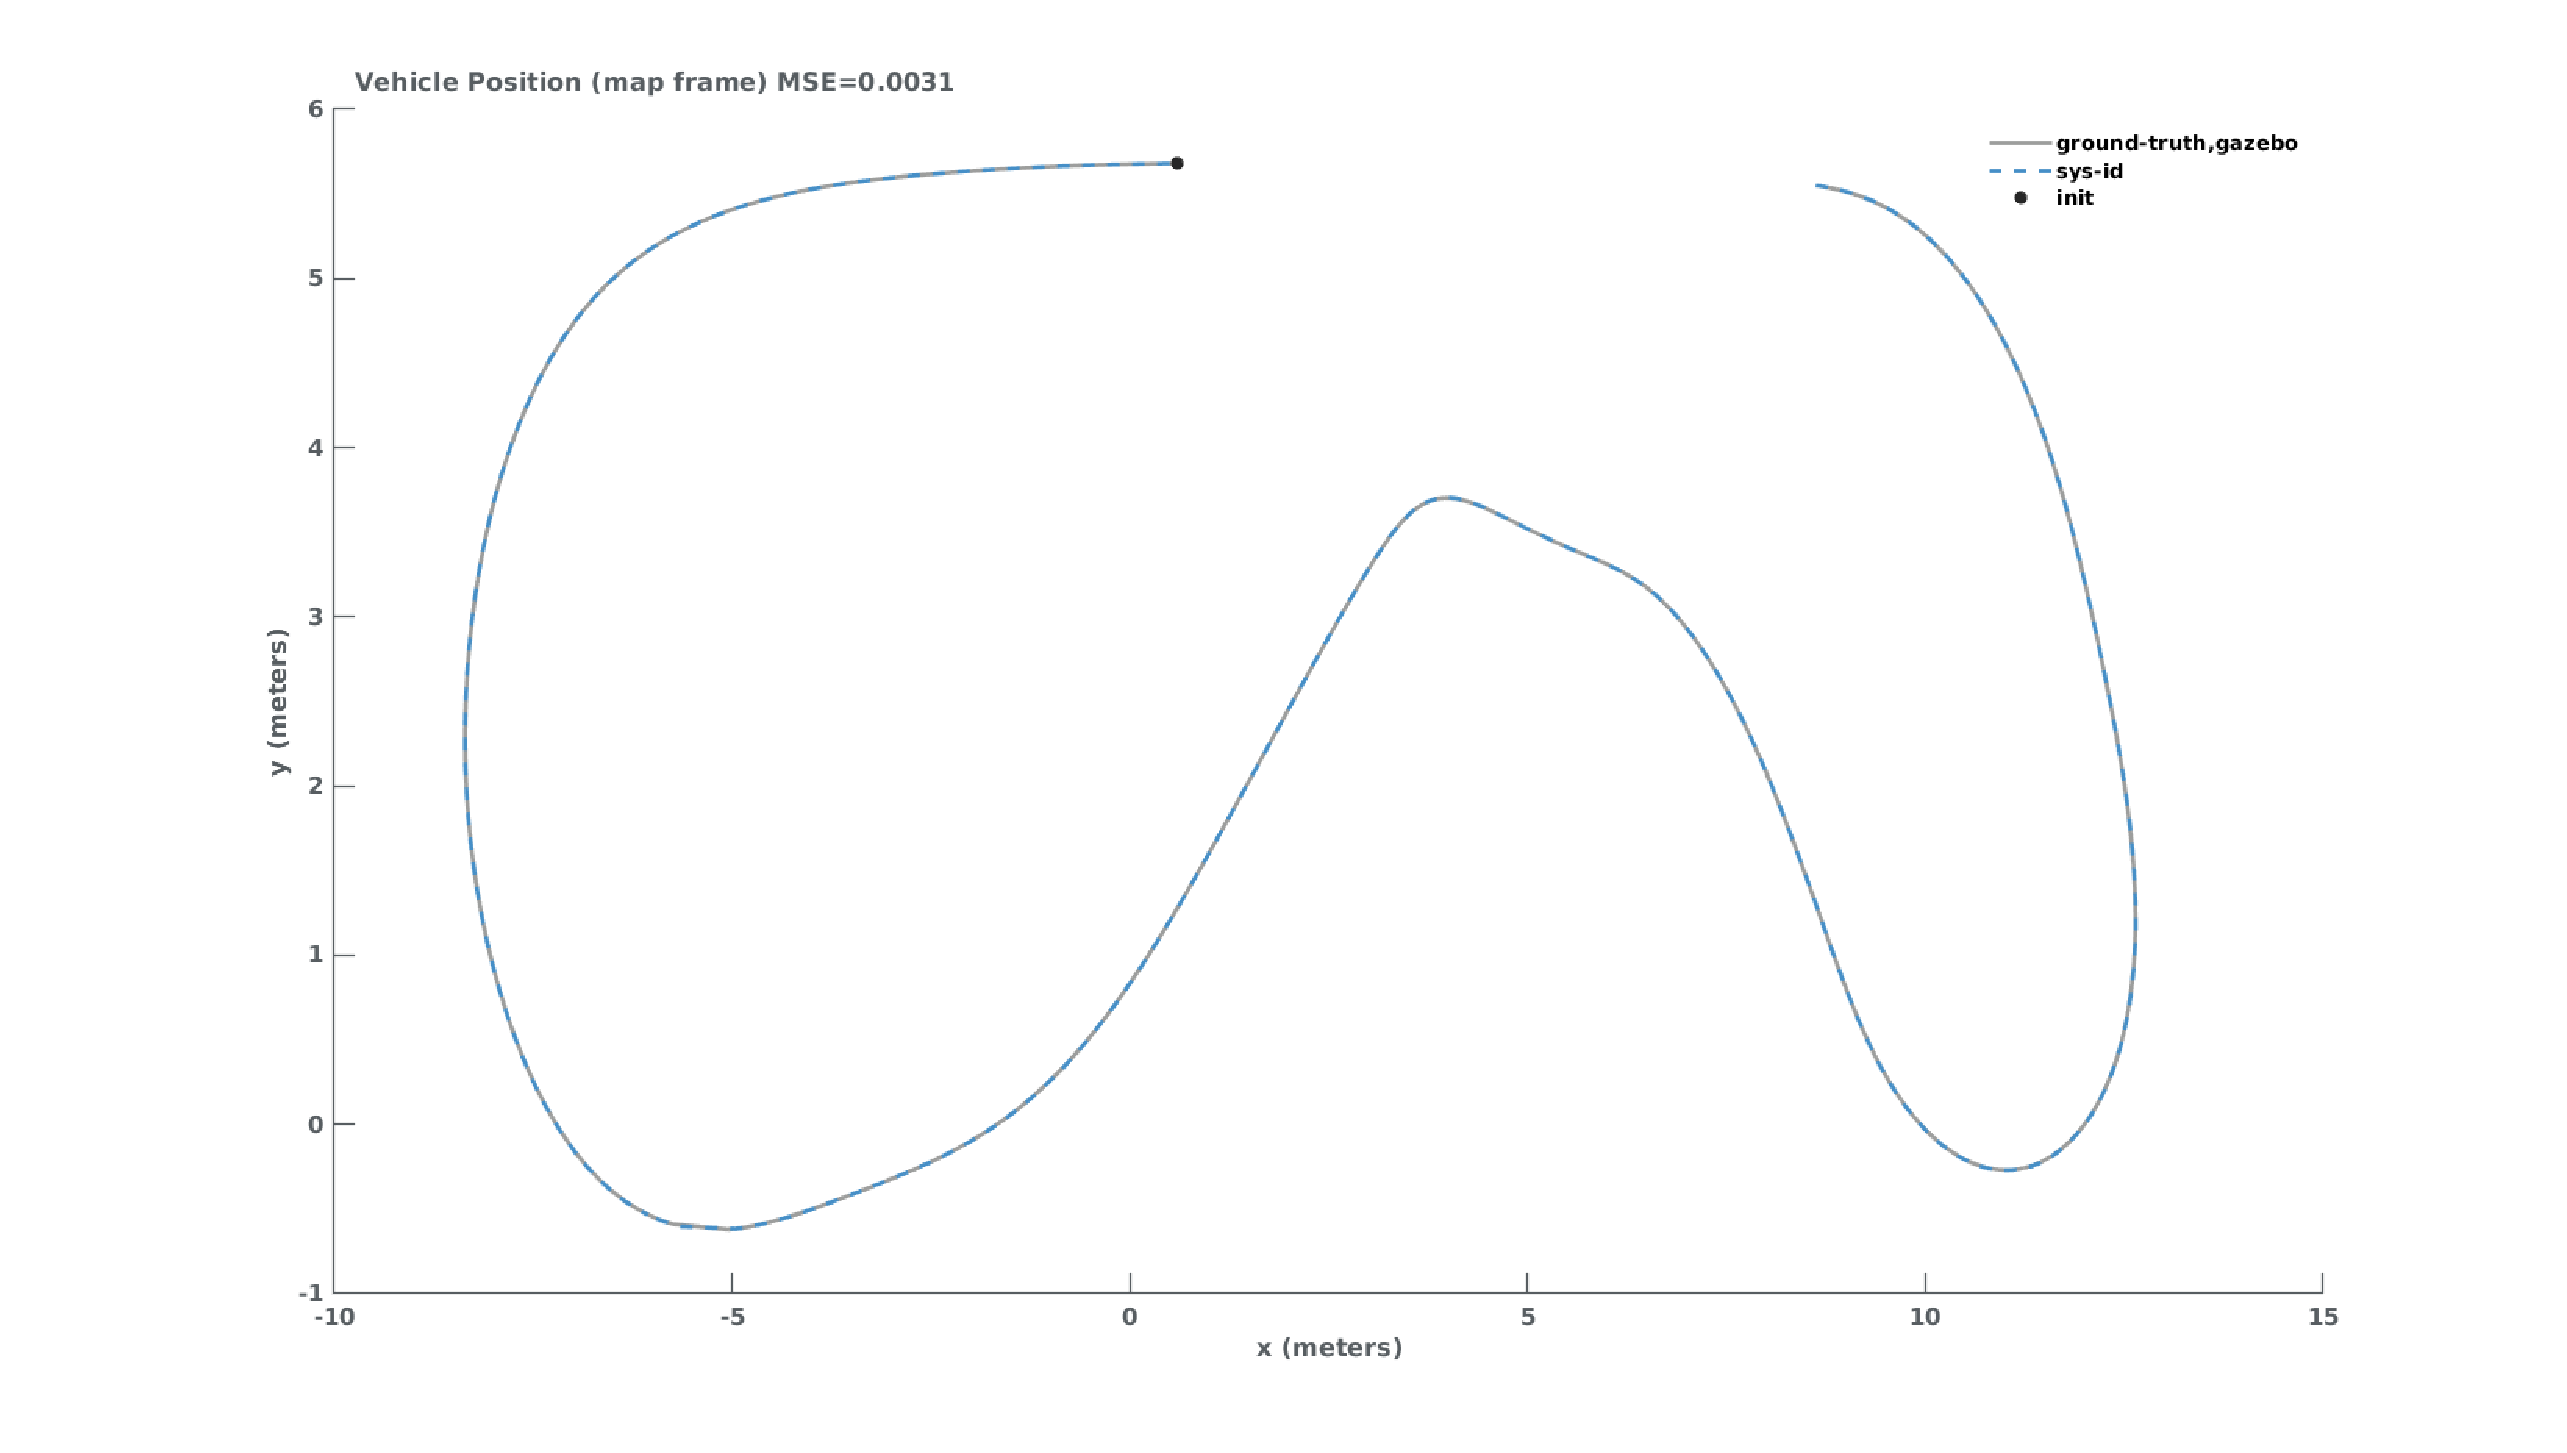
\includegraphics[width=0.7\linewidth]{figures/validation2.pdf}
%   \caption{Model validation for the F1/10 Hardware Model using data collected from a manual set of experimental runs. \emph{Init} corresponds to the starting position of the vehicle in the considered experiment.}
%   \label{fig:validation}
% \end{figure}%


%In order to build and assure the safety of our system at runtime, we perform the following steps. First, we construct a mathematical model of the F1/10 car's physical dynamics using system identification techniques. We then deploy one of our four trained machine learning or \emph{learning enabled controllers} (LECs) into the control architecture. These controllers are: two Imitation Learning controllers (IL) designed to mimic nominal driving behavior from data collected from a series of experiments of driving the vehicle manually, and two Reinforcement Learning controllers (RLc) that synthesize control policies through trial and error. At runtime, using the mathematical model that we obtained through system identification and our real-time reachability algorithm, we compute the reachable set of states from the current state and the control input given by our LEC, for a specified reach time. During the construction of the reachable set, we perform safety checking in order to gauge whether the reachable set of states intersects with known obstacles or the walls defining the track environment. Lastly, based on the results of the safety checking, we design a simplex strategy to maintain safe operation of the F1/10 model. 

\section{Controller Construction}

Modern data-driven or machine learning methods have become increasingly scalable and efficient in dealing with complex problems in numerous contexts. In this section, we provide a high-level introduction to imitation learning and reinforcement learning and describe the construction of the controllers used within our simplex architecture.

\subsection{Imitation Learning}

Imitation learning (IL) seeks to reproduce the behavior of a human or domain expert on a given task \cite{Hussein2017ImitationL}. These methods fall under the branch of \textit{Expert Systems} in AI which has seen a surge in interest in recent years. The increase in demand for these approaches is spurred on by two main motivations. (1) In many settings, the number of possible actions needed to execute a complex task is too large to cover using explicit programming. (2) Demonstrations show that having prior knowledge provided by an expert is more efficient than learning from scratch \cite{Hussein2017ImitationL}.

One of the most common imitation learning methods is \textit{Behavior Cloning}, whereby a controller is constructed by learning a mapping from sensor-action pairs collected either from a baseline controller or through human-in-the-loop control. While these approaches have demonstrated great efficacy in fixed contexts, there have been concerns about their ability to generalize to novel contexts where the operating conditions are different from those seen during training \cite{Majumdar2017}.
%This paradigm was first introduced to train a multilayer perceptron tasked with enabling a modified van to navigate paths at speeds of up to 20 miles an hour \cite{pomerleau1989alvinn}. The work was later replicated with a convolutional neural network architecture in \cite{bojarski2016end} with great success. 
In this work, we utilize behavior cloning to train two neural network controllers to produce steering angles from sensor inputs. The first controller is trained on camera-images and leverages an architecture used by Bojarski et al. to control a real-world autonomous vehicle \cite{bojarski2016end}. The second controller utilizes a much smaller neural network model and is trained on a discrete sampling of lidar distance measurements. This network allows for more fair comparisons to the reinforcement learning approaches. %\todo{Our hypothesis is that controllers trained on images will experience greater challenges in zero-shot policy transfer? Maybe not a hypothesis but it would be an interesting result from our analysis}

\subsubsection{Vision-Based Navigation (VBN)}
%\diego{Isn't the lidar behavior cloning and E2E controller too? End to end means that the output of the controller is solely based on the inputs from the sensors/environments, right?. I would change the name of this subsection. And I guess RL (in this sense) it is also E2E.}
%Vision-based perception systems for autonomous driving can be broadly classified into two categories: mediated-perception approaches and end-to-end, or behavioral-reflex, approaches \cite{DeepDrive2015}. Mediated perception approaches involve multiple sub-components for recognizing objects relevant to the driving task, that are then combined into a world representation utilized by a decision manager to issue control actions. In contrast, end-to-end approaches compute a direct mapping from images to control actions \cite{DeepDrive2015}. While end-to-end approaches have proven to be an elegant and effective reduction of a complex system, they are "black box" in nature which makes them difficult to debug. Within the context of this manuscript, we opted to use end-to-end approaches because of their straightforward incorporation within the simplex architecture, and they allow us to evaluate our safety regime more plainly.

%Such systems are typically constructed using data where a human, or baseline controller, controls the system during a series of experiments. The control commands and corresponding images are then used to train a convolutional neural network to fit this non-linear mapping \cite{DirectPerception2019,AlexNet2012}. 

% Mediated-perception approaches involve multiple independent components for detecting objects relevant to the driving task such as lanes, objects, traffic lights, pedestrians, and other vehicles. Each component then returns its observations to a decision manager that controls the vehicle.

% Accordingly, given unexpected behavior, it is hard for the designer to find the source of errant behavior \cite{VisionBased2019}.


%End-to-end approaches have demonstrated efficacy in simple tasks such as lane following, and although they represent an elegant idea, these approaches struggle to be robust in complex traffic and driving scenarios  \cite{DeepPiCar2017}. While mediated approaches are more transparent, making them more accessible to inspection and debugging, end-to-end methods are largely "black-box" in nature. Thus, current state-of-the-art systems typically make use of mediated approaches in autonomous vehicle applications. However, these systems exhibit considerable complexity as it relates to the perception problem by detecting redundant objects that may not be useful in driving control decisions \cite{DeepDrive2015}. 

Since the seminal work of Krizhevsky et al. \cite{AlexNet2012} in the ImageNet Large Scale Recognition Challenge, \emph{Convolutional Neural Networks} (CNNs) have revolutionized the field of computer vision. Within the context of autonomous vehicles, CNNs have demonstrated efficacy in being used to enable driving tasks such as lane following, path planning, and control, simultaneously, by computing steering commands directly from images \cite{DeepDrive2015}. In \cite{bojarski2016end}, Bojarski et al. utilized a CNN architecture called DAVE-2 to control a 2016 Lincoln MKZ for over 10 miles in a series of successful on-road tests. For this reason, we selected this architecture for our experiments. 

The data we used to train DAVE-2 was collected from set of simulation experiments where the sensor-action pairs were generated by a path tracking controller optimized to keep the F1/10 in the center of the track. Such an environment is shown in \figref{fig:reachset}. The path-tracking controller was designed using the well-known pure-pursuit algorithm \cite{coulter1992implementation}. To ensure robustness, we augmented these experiments with a set of configurations in which the F1/10 deviated from the center of the track and recorded the actions that the path tracking controller enacted to return to the nominal path. In total, the dataset consists of 5000 images.  To investigate the use of our simplex architecture in novel contexts, the training data was collected in the absence of obstacles.
 


% \begin{figure}[!htbp]
%   \centering
%     % \hspace*{-8mm}  
%     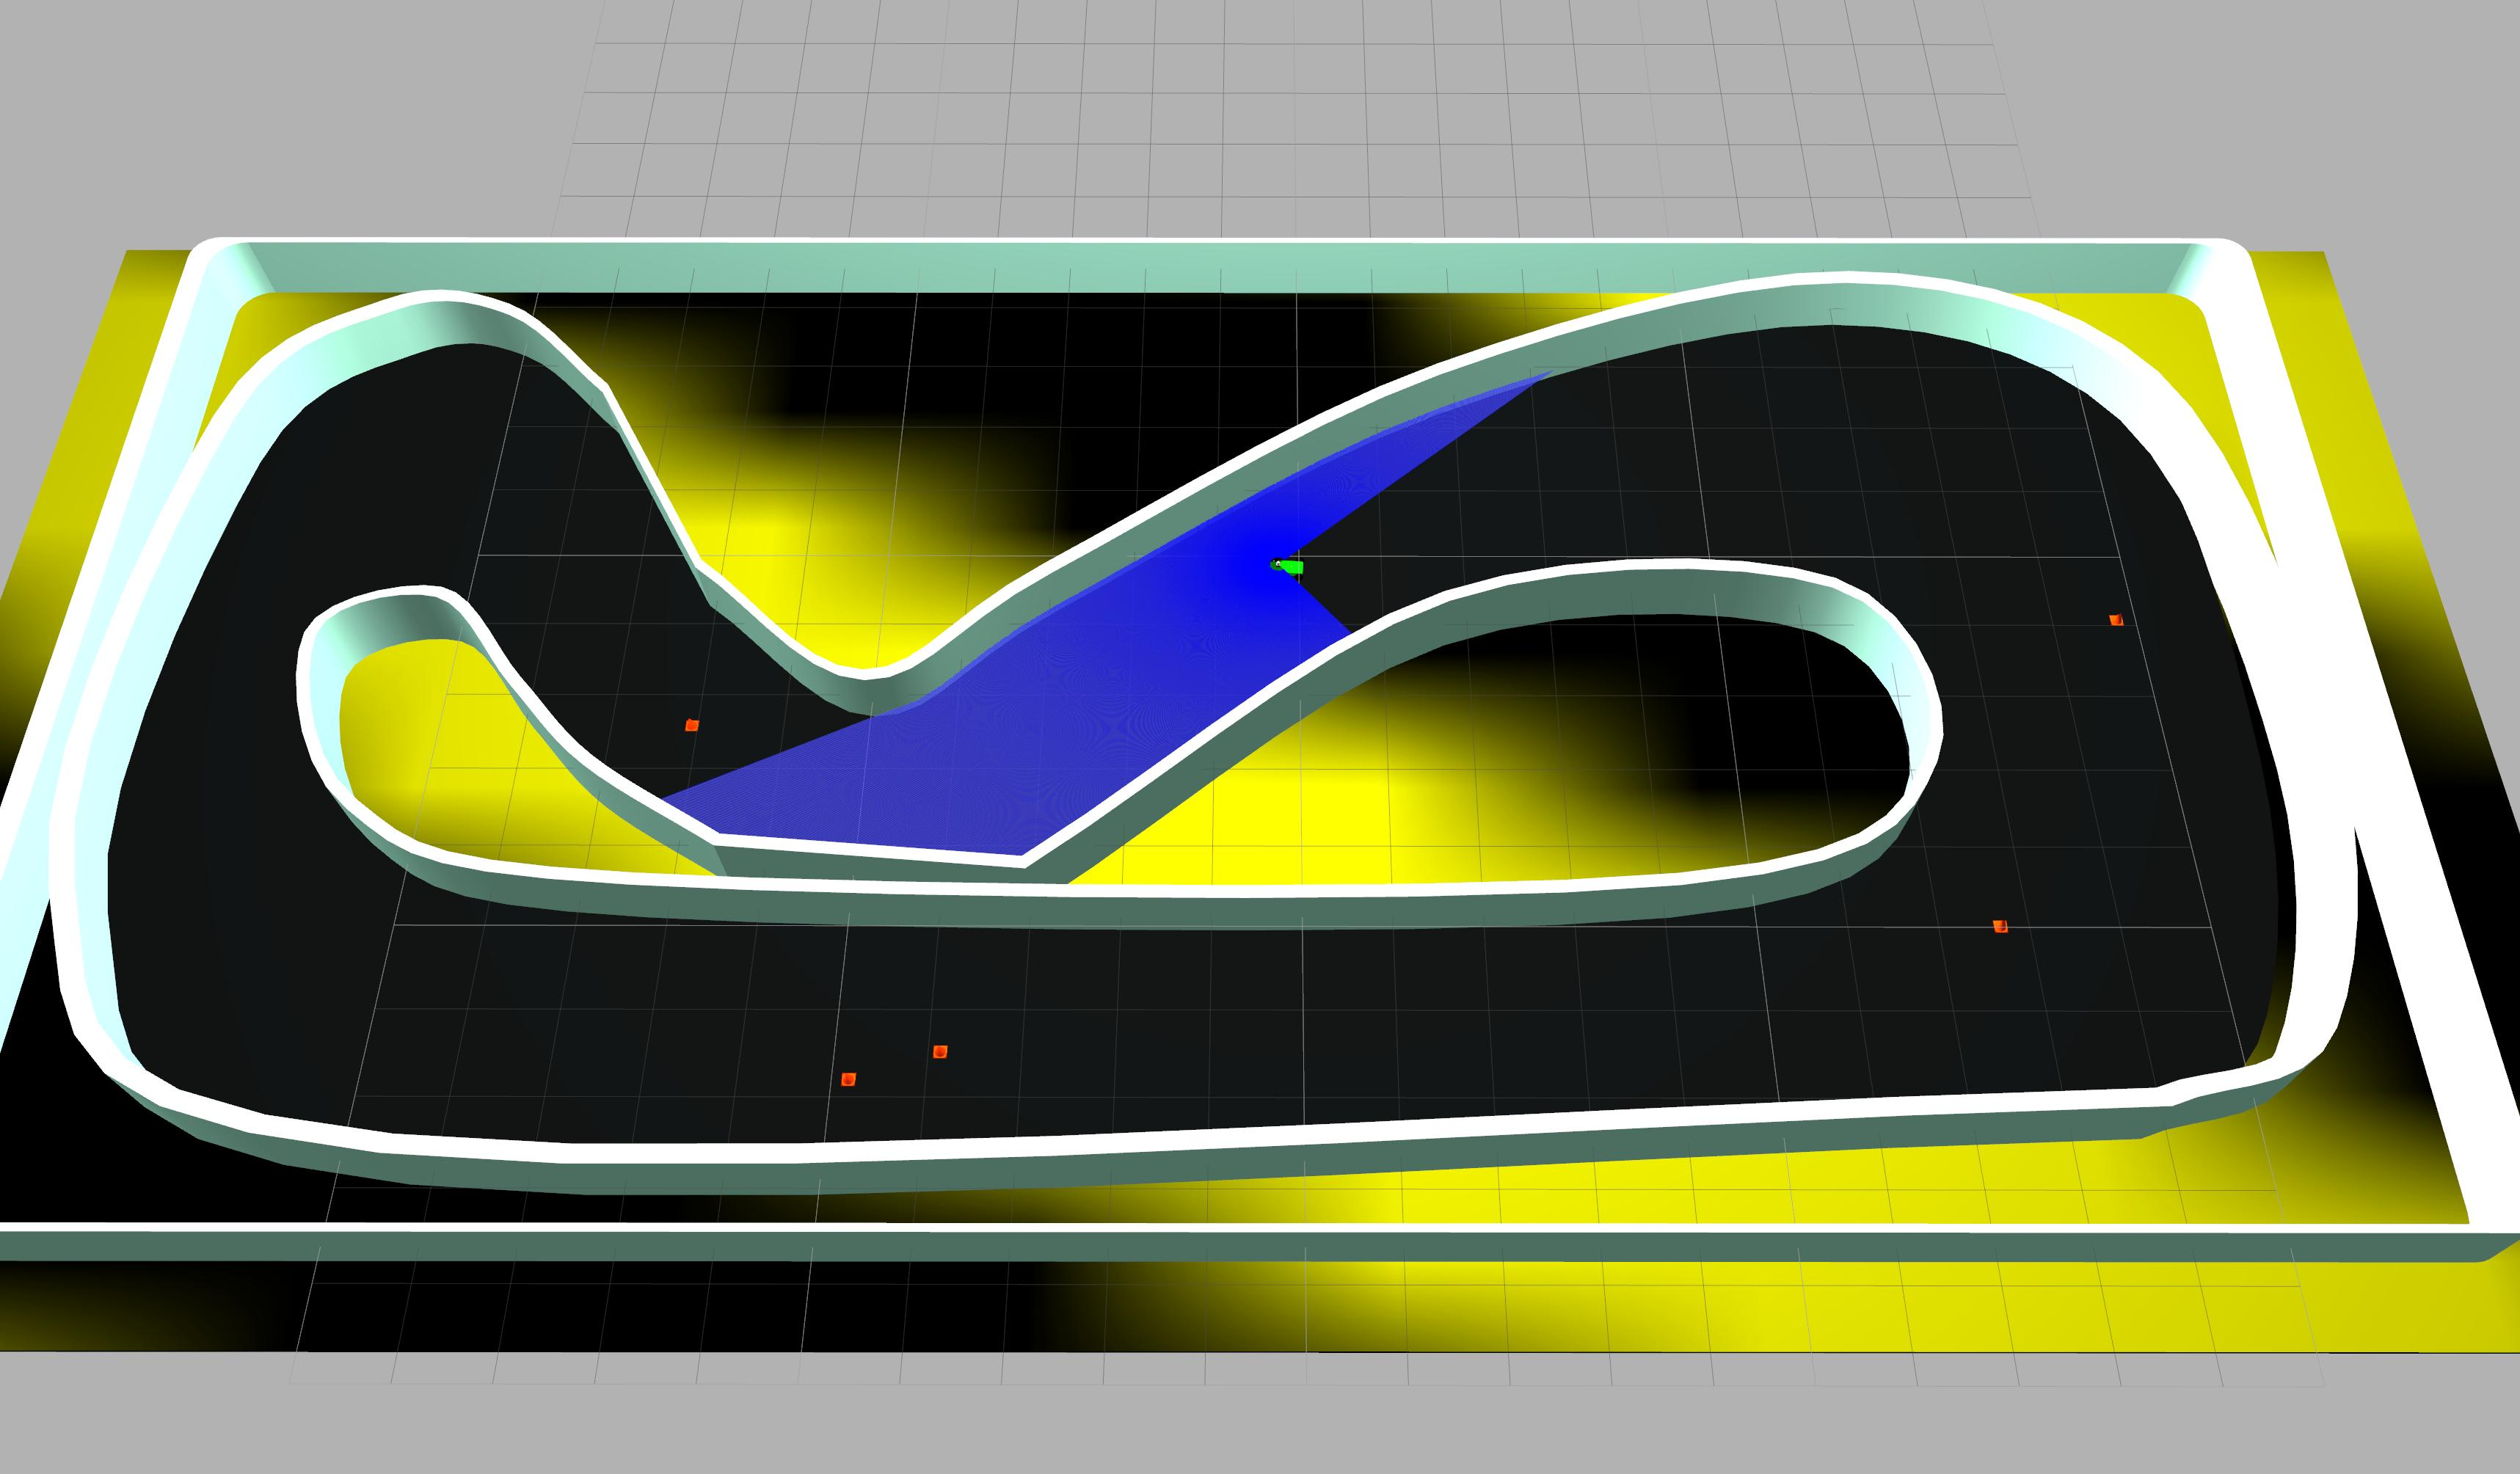
\includegraphics[width=0.65\textwidth]{figures/gazebo.jpg}
%   \caption{Simulation of F1/10 Car and obstacles using Gazebo.}
%   \label{fig:racetrack}
% \end{figure}

\subsubsection{Lidar Behavior Cloning (LBC)}
\label{sec:lidar cloning}
The second network considered for behavior cloning was a standard multi-layer perceptron network that consists of an input layer, 2 fully connected hidden layers of 64 nodes with ReLU activation functions, and a fully connected output layer with a $\tanh$ activation function. The input layer accepts nine range values collected from the LiDAR at $-90^{\circ}$, $-60^{\circ}$, $-45^{\circ}$, $-30^{\circ}$, $0^{\circ}$, $30^{\circ}$, $45^{\circ}$, $60^{\circ}$, and $90^{\circ}$ from forward. The range values are clipped between $[0m, 10m]$. The data used to train this controller was collected in the same fashion as the end-to-end regime. 


%We divided the driving task into five distinct categories based on the images observed from our on-board camera. The classes we utilized are: left, weak left, straight, right, and weak right. The classes are displayed in \ref{fig:classes}. The corresponding control inputs are ($\delta = 0.51$), ($\delta = 0.10$), $(\delta = 0.0)$, ($\delta=-0.51$), and ($\delta= -0.10$) respectively.

%\begin{figure}%[ht]
%  \centering
%    % \hspace*{-8mm}  
%    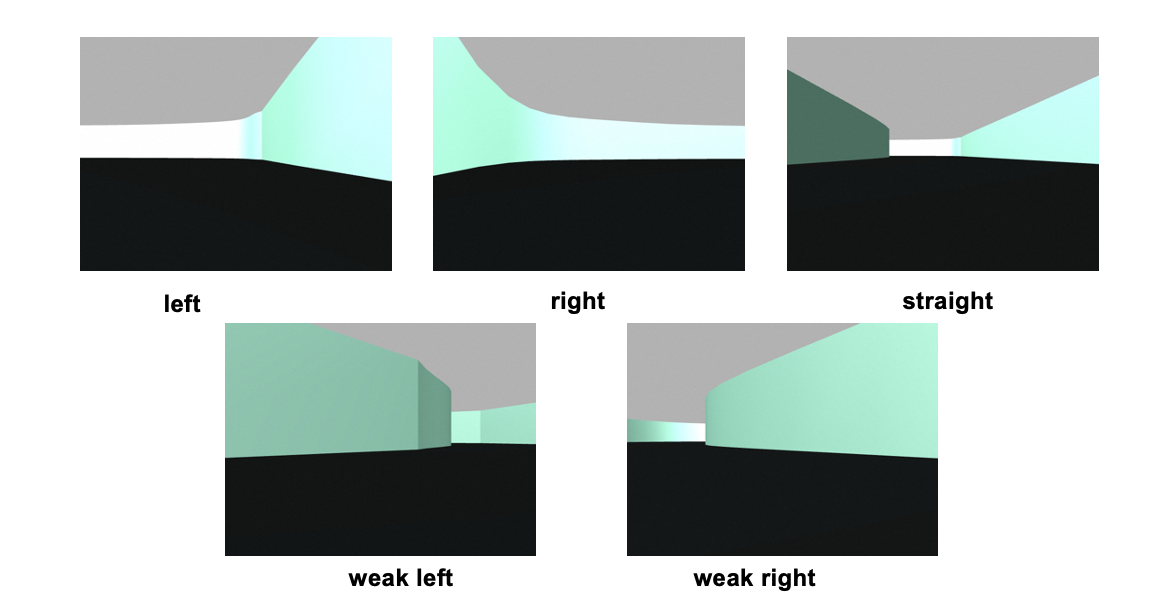
\includegraphics[width=0.7\linewidth]{figures/classes.png}
%   \caption{Classes used in the the end-to-end classification task.}
%  \label{fig:classes}
% \end{figure}

 %\url{https://github.com/pmusau17/Platooning-F1Tenth/tree/master/src/computer_vision}}.
%Additionally, in order to investigate the use of our simplex architecture in novel contexts, the neural network was trained in the absence of obstacles within the racetrack environment.



\subsection{Reinforcement Learning Control}
Reinforcement Learning and Deep Reinforcement Learning (both referred to as RL) are branches of machine learning that focus on software agents learning to maximize rewards in an environment through experience. Their essence is similar to training a dog to do tricks by giving it treats when it performs the desired task. In doing so, the agents obtain a policy that maps the systems states with corresponding actions in an optimal fashion. These approaches have achieved state-of-the-art performance on many high-dimensional control tasks \cite{lillicrap2015continuous, schulman2017proximal, mania2018simple, haarnoja2018soft}. Despite the growing success, RL approaches are mainly leveraged within simulation due challenges of ensuring safe training processes for real-world systems, designing reward functions that deal with noisy and uncertain state information, and ensuring trained controllers are able to generalize beyond fixed scenarios \cite{dulac2019challenges}. While training a controller in simulation and moving into the real world, a process known as \emph{sim2real} transfer, is possible, it often results in undesired, poor, and/or dangerous behavior \cite{jang2019ICCPS, kadian2019we}.

In this paper, we highlight how using this simplex architecture can prevent dangerous behavior when transferring a trained policy from simulation to the real world or to a novel context.
To demonstrate the effectiveness of this method, we trained two well-known state-of-the-art reinforcement learning algorithms, an off-policy deep reinforcement learning algorithm known as \emph{Soft-Actor-Critic} (SAC), \cite{haarnoja2018soft}, and an on-policy RL algorithm, known as \emph{Augmented Random Search} (ARS), \cite{mania2018simple}. %The policies were trained in our simulator with hyperparameters listed in Appendix \ref{app:rl_training}.
In line with the imitation learning experiments, the agents were trained on the racetrack shown in \figref{fig:reachset} with no obstacles and no backup controller. For both algorithms, the agent optimizes performance on a dense reward function that assigns a positive reward for counterclockwise progress around the track. The reward is calculated using a reference path that runs through the middle of the track. The value of the reward is the positive arclength between the previous closest point and the current closest point along the path. This reward function encourages the agent to complete as many laps as possible as quickly as possible.

After training to an optimal policy\footnote{All of the training scripts that enabled this work will be provided upon the completion of the double-blind review process.}, the control policies were locked and used without any further augmentations for the experiments described in Section \ref{sec:experiments}. This method of locking the control policy and using it in a different environment without further augmentations is often referred to as \emph{zero-shot policy transfer}.


\subsubsection{Soft Actor Critic}
(SAC) was first introduced 2018 as an improvement to \emph{Deep Deterministic Policy Gradient} (DDPG) that tackled RL's major challenges: high sample complexity and brittle convergence properties, i.e. a heavy dependence of hyperparameters being "just right" in order to effectively learn \cite{haarnoja2018soft}. They address these issues using a maximum entropy reinforcement learning framework. Instead of allowing the agent to explore the environment randomly while training, the actions are selected in a way that maximizes the number of unique training samples that are collected. Thus, the sample complexity is reduced because the process of collecting unique training samples is more efficient. Additionally, the agent is more likely to converge on the optimal control policy even when the hyperparameters are not tuned "just right."

In this work, the SAC controller was trained
%using hyper-parameters given in\ref{app:rl_training} and utilized 
using the architecture described in Section~\ref{sec:lidar cloning}. During the training process, we halted training to evaluate the agent's performance after every 500 training steps. The performance is then measured by how many laps the agent can complete within 100 seconds. This is more than enough time to complete 2 laps in the training track. The evaluation is repeated up to 10 times and training stops when the agent is able to complete at least 2 laps 10 times in a row. Once the agent is able to complete at least 2 laps 10 times, the training process is halted and control policy is saved for our experiments.

\subsubsection{Augmented Random Search} 
(ARS) was first proposed in 2018 as a random search method for training static, linear policies for continuous control problems \cite{mania2018simple}. Their simple method was able to match state-of-the-art sample efficiency on the benchmark MuJoCo locomotion tasks\footnote{These benchmark tasks are described in more detail at \url{https://gym.openai.com/envs/\#mujoco}}, demonstrating that deep neural networks might not be necessary for some complex control tasks. We chose to highlight this RL algorithm because %in comparison to algorithms such as Proximal Policy Optimization (PPO) \cite{schulman2017proximal} or Soft Actor-Critic (SAC) \cite{haarnoja2018soft}, ARS can achieve optimal results with simpler reward functions. Successfully training a PPO or SAC agent often requires considerable reward shaping or the use of a gate-based reward that is more difficult to construct within the simulation environment.
it allowed us to experiment with a different control architecture. Both LBC and SAC are the same NN architecture differentiated by how the networks are trained. In contrast, ARS focuses on the use of a linear policy, i.e. a weight matrix. Instead of passing the input through multiple layers with non-linear activation functions as is done in the NN controllers, the input is multiplied by a single weight matrix to generate the control output. %Thus, the control output can be calculated much more quickly than with a NN, so we can run the controller at faster rates. This allows us to push the bounds of our reachability stuff. \nate{<-- I wrote this explanation, but idk if it's a good one.}

Similar to the SAC architecture, the output control signal of the ARS policy, $\delta = \pi(s)$, is the desired steering angle clipped between $\pm34^{\circ}$. However, the input, $s$, consists of $271$ lidar range values, clipped between $[0m, 10m]$, collected from between $\pm90^{\circ}$ from forward. During the training process, we halted training to evaluate the agent's performance after every batch of rollouts. The performance is then measured by how many laps the agent can complete within 50 seconds. The evaluation is repeated 5 times and training stops when the agent is able to complete at least 2 laps 5 times in a row. Once the agent is able to complete at least 2 laps 5 times, the training process is halted and control policy is saved for our experiments. We changed the cutoff requirements for this agent because when we trained the agent with the same requirements as the SAC agent, the ARS agent met the requirement very quickly, but the resulting policy was very inefficient. %\nate{Do we want to retrain the SAC agent to have the same cutoff as ARS? or is this ok?}



% The control policy uses the forward-facing semi-circle of collected lidar range data to determine the desired steering angle by way of a linear policy, i.e. a weight matrix. 
\section{ONLINE REACHABILITY COMPUTATION}

Before outlining the algorithm, let us define two key terms relevant to our approach.\smallskip

\begin{definition}%
(REACHTIME). The reachtime, $T_{reach}$, is the finite time horizon for computing the reachable set.
\end{definition}%\smallskip
\begin{definition}%
(RUNTIME). The runtime, $T_{runtime}$, is the duration of (wall) time the algorithm is allowed to run.
\end{definition}% \smallskip
%With that, the real-time reachability algorithm works as follows.
 Using the dynamics model obtained for the F1/10, the crux of the real-time reachability algorithm is computing the set of reachable states from the current time $t$ up until $(t+T_{reach})$. The algorithm utilized within this work is based on mixed face-lifting, which is part of a class of methods that deal with \textit{flow-pipe construction} or \textit{reachtube computation} \cite{Johnson2016}. This is done using snapshots of the set of reachable states that are enumerated at successive points in time. To formalise this concept, we define the reachable set below.
\smallskip
\begin{definition}%
(REACHABLE SET). Given a system with state vector $\textbf{x}(t) \in \mathbb{R}^n$, input vector $\textbf{u}(t) \in \mathbb{R}^m$, and dynamics $\dot{\textbf{x}}(t)=f(\textbf{x}(t),\textbf{u}(t))$, where $t$ is time, and the initial states $\textbf{x}_0 = \textbf{x}(0)$ and inputs $\textbf{u}_0 = \textbf{u}(0)$ are bounded by sets, $\textbf{x}_0 \in \chi_0$, $\textbf{u}_0 \in \mathnormal{U}$. The reachable set of the system for a time interval $ t \in [0,T_{reach}]$ is:%
%
\begin{equation*}%
    \mathnormal{R}_{[0,T_{reach}]} = \big \{ \psi(\textbf{x}_0,\textbf{u}_0,t) \ \big| \ \textbf{x}_0 \in \chi_0, \ \textbf{u}_0 \in \mathnormal{U}, \ t \in [0,T_{reach}\big]\},%
\end{equation*}%
%
\noindent where $\psi(\textbf{x}_0,\textbf{u}_0,t)$ is the solution of the ODE at time $t$ with initial state $\textbf{x}_0$ under control input $\textbf{u}_0$.\todo{may want to add a footnote / set of assumptions on this, e.g., we don't actually use the ODE solution in the reachability [which is a feature/benefit], but in this definition may want to assume the solution exists, which if nonlinear, in general may not; assuming the odes are lipschitz continuous should be sufficient for the solution to exist}
\end{definition}%
\smallskip

\begin{figure*}[htbp]%[tb]
  \centering
  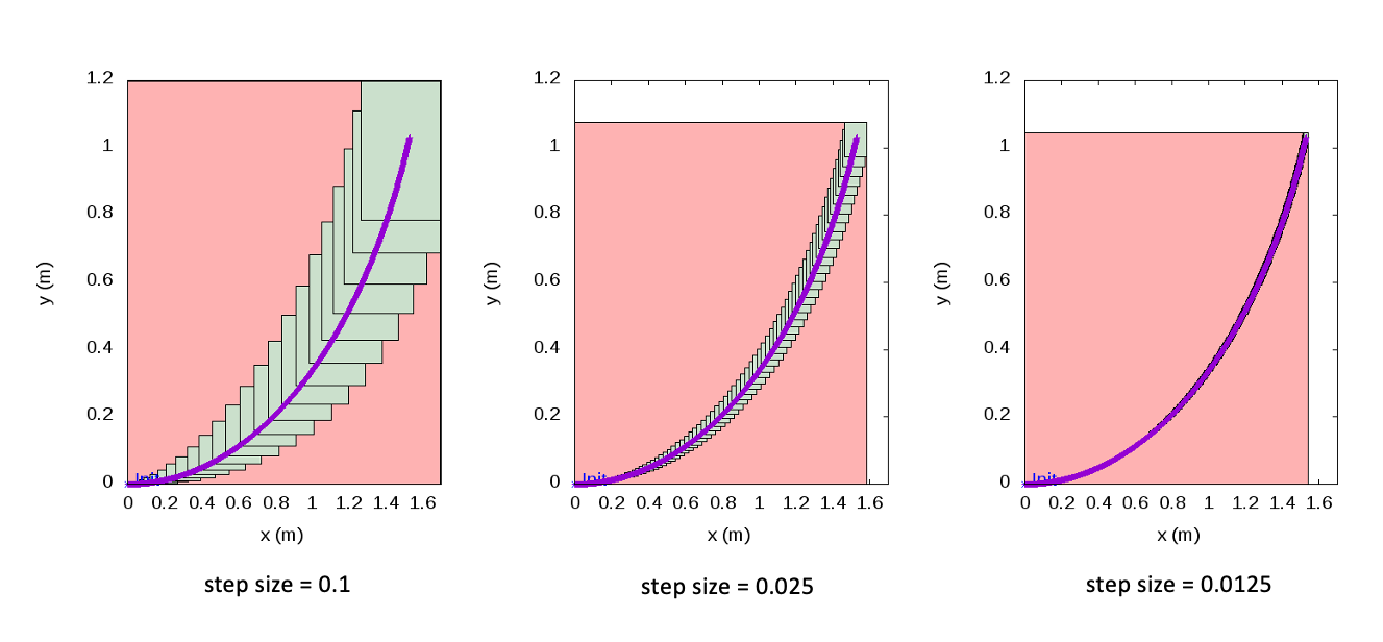
\includegraphics[width=0.90\linewidth]{figures/refinement_cropped.pdf}
  \caption{The real-time reachability algorithm always returns an over-approximation of the reachable set of states. The over-approximation error decreases with successive iterations, provided that there is enough runtime for re-computations. The above images demonstrate this aspect by simulating a left hand turn control action for a reachtime of two seconds. The green boxes represent the set of reachable states, the red rectangle represents the interval hull of the reachable states, and the purple points are points obtained from a simulation of the vehicles dynamics.}
  \label{fig:reach_refine}
\end{figure*}%
In general for nonlinear systems, it is not possible to obtain the exact set of reachable states $\mathnormal{R}_{[0,T_{reach}]}$, so we customarily compute a sound over-approximation such that the actual system behavior is contained within the over-approximation \cite{AlthoffNonlinear,Lin2020,Asarin2003}. The algorithm utilized in this work utilizes $n$-dimensional hyper-rectangles ("boxes") as the set representation to generate reachtubes \cite{Johnson2016}. Over long reachtimes, the over-approximation error resulting from the use of this representation can be problematic. However, for short reach-times, it is ideal in terms of its simplicity and speed \cite{Bak2014}. 
%\diego{There is a paper that formally reasons that computing the exact reachable set of nonlinear systems (bycicle model) is NP-hard... I could try to find it if we want to cite it, although not sure how important it is for the runtime verification since even if it was possible, it would be too computationally expensive to use it in this regime},

The over-approximation error and the number of steps used in generating the reachable set can be controlled by a reachtime step size $h$. This parameter defines the level of discretization of the time interval $[0,T_{reach}]$ and can be used to tune the runtime time of the reachability computation. Bak et al. leverage the step size to make the reachability algorithm amenable to the anytime computation model in the real-time scheduling literature \cite{Liu1991}. Thus, given a fixed runtime, $T_{runtime}$, we compute the reachable set $\mathnormal{R}_{[0,T_{reach}]}$, and if there is remaining runtime, we restart the reachability computation with a smaller step size. In both this work and \cite{Bak2014}, the step-size is halved in each successive iteration, leading to more accurate determinations of the reachable set. The relationship between the over-approximation error and the step size can be seen in \figref{fig:reach_refine}. We refer readers to the following papers for an in depth treatment of these procedures \cite{dang2000,Bak2014,Johnson2016}.



%$h$, used to discretize the time interval defined by the reachtime. In designing the technique, Bak et al. leveraged this step size to tune the over-approximation error as well as the runtime, $T_{runtime}$, associated with computing the reachable set. In doing so, the approach becomes amenable to the   As done in \cite{Bak2014}, 





 %A high level overview is presented in Algorithm~\ref{alg:algo_rtreach}, and we refer readers to the following papers for an in depth treatment of these procedures \cite{}. 


\section{SAFETY CHECKING}

We define the notion of safety considered in this work below. \smallskip
%work consists of checking for intersections between the set of unsafe states and $\mathnormal{R}_{[0,T_{reach}]}$. We define
\begin{definition}%
(SAFETY). Let $\Lambda$ represent the set of unsafe states. A system is considered safe over the finite time horizon, $T_{reach}$, if  $\mathnormal{R}_{[0,T_{reach}]} \  \cap \ \Lambda \ = \ \emptyset$. Here, $\Lambda$, consists of all static obstacles within the environment and the boundaries of the racetrack.
\end{definition}%\smallskip



\begin{algorithm}[htbp]%
\DontPrintSemicolon 
INITIALIZE{
\\
\textbf{Input:} $\chi_0,\mathnormal{U},T_{reach}, T_{runtime}$ \\
\textbf{Output:} $safe$ (boolean)
}

\vspace{2mm}

REACHABILITY ANALYSIS\\
$elapsedTime = 0$\;
$T_{remaining} = T_{runtime}$\;
\While{$T_{remaining}$>0} {
    %\% Construct the Reachable Set\;
    $safe = $ true\;
    $\mathnormal{R}_{[0,T_{reach}]}= constructReachSet(\chi_0,\mathnormal{U},T_{reach},h)$\;
    %\% Check for intersections with unsafe set\;
    \If{$\mathnormal{R}_{[0,T_{reach}]} \cap \Lambda \neq \emptyset $}{
    $safe = $ false\;
    }
    $elapsedTime$ = computeElapsedTime()\;
    $nextIterationEstimate$ = estimateNextIterationRuntime($elapsedTime$)\;
    $T_{remaining} = T_{runtime} -elapsedTime - nextIterationEstimate$\;
    $h = h /2$\;
    
    
    
}
\textbf{return:} $safe$
\caption{Real-time Reachability Algorithm}
\label{alg:algo_rtreach}
\end{algorithm}%

Each obstacle within the environment can be described by a bounding-box, and the racetrack boundaries can be characterized by a list of finely separated points. These representations are then converted into their hyper-rectangle formulations that make up $\Lambda$. \figref{fig:reachset} provides a visualization of the obstacles, and \figref{fig:lab_setup} displays our discretization of the racetrack. If there are no intersections between $\mathnormal{R}_{[0,T_{reach}]}$ and $\Lambda$, then we conclude that the system is safe. However, since our approach computes an  over-approximation of $\mathnormal{R}_{[0,T_{reach}]}$, it may lead to conservative observations of unsafe behavior. This occurs when the error in the over-approximation of $\mathnormal{R}_{[0,T_{reach}]}$ results in intersections with the set of unsafe states, but these intersections would not occur with the exact reachable set. By refining the reachable set in successive iterations, our regime seeks to mitigate the occurrence of false positives.  


There were two chief considerations in the anytime implementation of the safety checking procedure. These constitute the novel aspects of our algorithm. The first was with respect to the overall soundness of our approach, and the second was related to the real-time nature of our scheme. For the results of the verification to be sound, the safety checking process must be carried out in its entirety before a safety result is issued. At the same time this requirement must be balanced alongside the real-time stipulation that tasks operate within pre-defined and deterministic time spans. Thus, our implementation needed to ensure that fulfilling soundness properties admitted a low-likelihood of missing timing deadlines.

Ideally, to ensure there were no missed deadlines, we would build our system in a \emph{Real-Time Operating System} (RTOS), which allows for the specification of task priorities so that they are executed within established time frames. However, our implementation did not make use of an RTOS, instead depending on native Linux and ROS to handle task management. To combat this shortcomming and reduce the number of missed deadlines, we utilized a method of estimating how long it will take to compute the next reachability loop.  If our estimate exceeds the remaining allotted time, the process terminates. There is an inherent tradeoff between the conservativeness of our runtime estimates and the conservativeness of the resulting reachable set. In this work, we chose to maximize the number of iterations used in constructing the reachable set. However, our experiments demonstrate that we were successful in minimizing the number of missed deadlines during operation. The estimation process is discussed more formally below.


%\todo{relate PMD to mean runtime. reducing the conservativeness of our estimation increases both}



%There were two chief considerations in the anytime implementation of the safety checking procedure. These constitute the novel aspects of our algorithm. The first was with respect to the overall soundness of our approach, and the second was related to the real-time nature of our scheme. For the results of the verification to be sound, the safety checking process must be carried out in its entirety before a safety result is issued.  At the same time we need to ensure that fulfilling this requirement admits a low-likelihood of missing timing deadlines and that the execution of the algorithm consistently occurs within the pre-defined runtime. To satisfy both requirements, we modify the algorithm presented in \cite{Bak2014} to include an estimate of how long an additional iteration of the reachability and safety checking process would take. This is based on observing how long the current iteration takes and reasoning about the number of hyper-rectangles that would be involved in the next iteration. If the remaining runtime is less than our estimate, then we terminate the computation and use the current safety result.


%The basic requirement for real-time systems is that tasks operate within pre-defined and deterministic time spans. 


Let $k$ denote the number of hyper-rectangles used in representing the reachable set. $k$ is characterized by the following equation: $k = T_{reach} / h$.\footnote{We begin the flow-pipe construction with an initial time step of $h = T_{reach}/10$.} Since in each successive iteration we decrease the step size by half, the number of hyper-rectangles that make up $\mathnormal{R}_{[0,T_{reach}]}$ doubles. Thus, the complexity of the safety checking process is $O(2^k)$.\footnote{This analysis neglects consideration of the obstacles and the points used to represent the racetrack boundaries. Since these do not change between iterations, reasoning only about the hyper-rectangles is sufficient.} Therefore, we can estimate that a subsequent iteration of the algorithm will take twice as long as the current one and bloat this estimate to be conservative. To ensure that our estimates are accurate in our implementation, rather than deriving $\mathnormal{R}_{[0,T_{reach}]}$ and then checking whether or not the system has entered an unsafe scenario, the safety checking is done during the computation with intermediate hyper-rectangles as outlined in \cite{Bak2014}. This prevents us from needing to dynamically store the reachable set and allows us to restart the computation sooner if an unsafe state is detected. A high-level overview is presented in Algorithm~\ref{alg:algo_rtreach}.%\footnote{The implementation details will be provided upon the completion of the double-blind review process.} 

%While our experiments demonstrated our approach missed deadlines, we still believe this work should be considered within \todo{words for "realm of real-time systems"}. 






\section{ROS Simplex Architecture}

\label{section:simplex}
The simplex architecture for the F1/10 is designed using ROS \cite{ROS}, and an overview of this design is shown in \figref{fig:simplex_arch}. 

There are two considerations that play a major role in design of the simplex architecture. The first consideration is the finite time horizon, $T_{reach}$, over which we are reasoning about safety. The second consideration is the amount of time, $T_{runtime}$, allocated for the computation of the reachsets. In our experiments, we utilized a reach time of 1.0 $s$. This was determined by empirical determinations of how long it took the F1/10 to come to a stop at speeds less than $1.5 m/s.$\footnote{The selection of velocities below 1.5 $ms$ was due to the size of our physical track that was ~13.08 meters in length. Races held by the F1/10 community are around typically 30-50 meters in length with large distances between the track walls.} The runtime allocated for the reachability algorithm was set at 25 $ms$ so as to ensure execution within a 20 $Hz$ control period.\footnote{The limiting factors are the Camera messages that are published at $20 \ Hz$.}  

Within this architecture, the primary sensors we rely on are a LiDAR and Stereo Labs' Zed Depth Camera. The messages from the LiDAR are published at $40 \ Hz$, and the Camera messages are published at $20 \ Hz$. Additionally, we rely on odometry information, published at $40 \ Hz$, in order to ascertain the state of the F1/10 vehicle. In our design, we decouple the control of the car's steering and throttle control. The steering control, $\delta$, is governed by the machine learning controller, and the throttle control is designed to maintain a constant speed, $u$, when the learning-based controller is in use. 

%The publishing rate of the decision manager within the simplex architecture is limited by the on-board camera, which captures images at 20 frames-per-second (FPS)\footnote{On the hardware platform, the camera can capture images as fast as 100 FPS. However, to keep the experiments consistent we limited the FPS to 20 FPS.}. Thus, as mentioned previously, we limited $T_{runtime}$, to $25 ms$ which corresponds to half the length of a control period. This was chosen based on empirical observations of the average execution time of the reachability algorithm, as well as a desire to ensure that the other parts of the decision logic could be successfully processed within a single control loop.

\begin{figure}[htbp]%
  \centering
  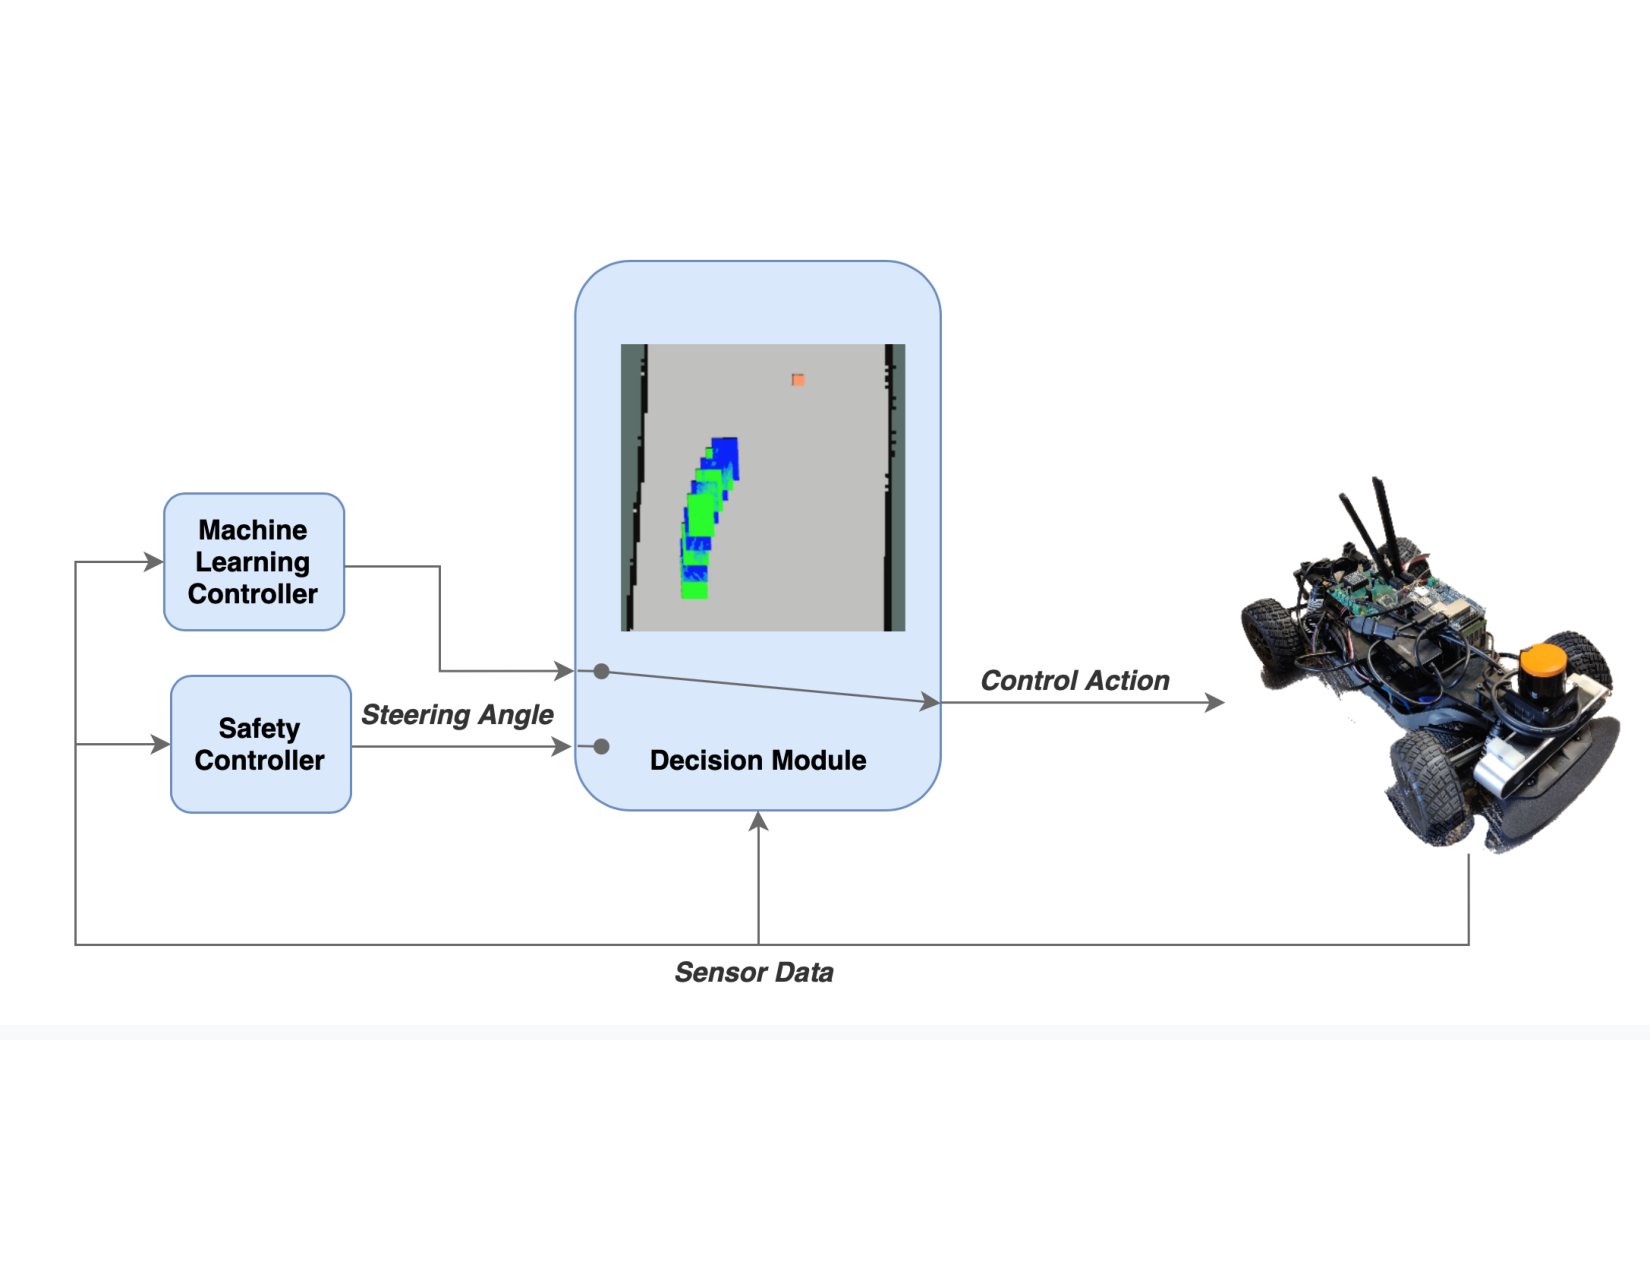
\includegraphics[width=0.8\linewidth]{figures/simplex_real.pdf}
  \caption{Overview of the Simplex architecture deployed on the F1/10 System as described in Section \ref{section:simplex}. The switching logic consists of monitoring the intersection between the F1/10 reachable set and the positions of static obstacles within the environment.}
  \label{fig:simplex_arch}
\end{figure}%

%\todo{Look into this a little more. See if I can come up with a more compelling justification }

In the traditional simplex architecture, for the system to be verified as correct, both the decision module and the safety controller must be verified \cite{Mehmood2021}. While this is straightforward for relatively simple controllers, it is significantly more challenging for many classes of controllers, especially when real-time execution is considered \cite{ivanov2020case}. In light of this, we opted not to develop a "formally verified" safety controller as is typically used within the simplex architecture. Instead, we selected a controller based on a gap-following algorithm optimized to avoid collisions with obstacles. A detailed description of the gap-following algorithm can be found in the following report \cite{otterness_2019}. It was primarily selected due to its robust collision avoidance ability and simplicity. Our primary focus was the evaluation of the real-time reachability regime, and our future work will consider verification of both the decision module and safety controller. 


\section{Experimental Evaluation}
\label{sec:experiments}
%\todo{Change this for emsoft}
%We evaluated our approach in an autonomous racing context inspired by the F1/10 Autonomous Racing Competition \cite{okelly2020}, where the vehicles are tasked with navigating a structured environment in a head-to-head race\footnote{The rules for the competitions can be found here: \url{https://f1tenth.org/race/rules-v2.pdf}}. During a race, vehicles are penalized for collisions with other race participants and with the track boundaries, and any serious collision results in disqualification. We denote the agent for which we are reasoning about safety as the ego vehicle. 

%During the race, we compute the set of reachable states for the ego vehicle and the other race participants over a finite time horizon. The lidar and stereo-camera are used for localization. The first parameter required by our regime is the finite time horizon over which we are reasoning about safety and in our experiments, this was determined by empirical determinations of how long it takes the F1/10 vehicle to come to a stop at various velocities. The ego vehicle traveled at a constant speed of 1.0 m/s, while the other race participants traveled at a constant speed of 0.5 m/s.\footnote{The selection of velocities was chosen out of a desire to promote interactions between the two vehicles and due to the size of our track that was ~13.08 meters in length. Races held by the F1/10 community are around typically 30-50 meters in length with large distances between the track walls.} A reach-time horizon of one second was determined acceptable to reason about safety for the ego vehicle and 0.8 seconds for the opponents.

%The second parameter required by our regime was the runtime allocated for the computation of the reachsets. Since the reachability regime utilized in this work is anytime in nature, increasing the allocated runtime allows for tigher appromiximations of the reachable set. An in-depth analysis of the reachability regime can be found in \cite{Bak2014}. In our experiments, we selected a wall-time of $10ms$, so as to ensure execution within a control period of $40 \ Hz$. 


% machine with We utilized two different laptop configurations to evaluate the simulation experiments. The first machine was a Dell Precision 7520 with 32GB RAM, an eight-core Intel Core i7-6820HQ CPU $@ 2.70\textrm{GHz}$ processor, and an Nvidia Quadro M2200 4GB graphics card. The second machine was 

Having described the details of our reachability algorithm, controller construction, and the simplex architecture construction, we now present the results of our empirical evaluations both in simulation and on the hardware platform. We ran our experiments on platforms running Linux (Ubuntu 16.04 LTS). The simulation experiments were conducted on a Dell XPS-15 (9570) with 32GB RAM, a six-core Intel Core i7-8750 $@ 4.1\textrm{GHz}$ processor, and an Nvidia GeForce GTX 1050Ti 4GB graphics card. The motivation for conducting simulation experiments stemmed from a desire to ensure fair comparisons over a large number of experiments and to promote reproducibility for those without hardware access.\footnote{A video demonstration can be found here: \url{https://streamable.com/zo4ocp}. All the code will be provided upon the completion of the double-blind review process.} The hardware experiments were done on an Nvidia Jetson-TX2 with a Dual-core Nvidia Denver 64-bit CPU (ARM), a quad-core ARM A57 Complex, and an NVIDIA Pascal Architecture GPU with 256 CUDA cores. The latter configuration validates our claims that our safety architecture admits minimal resource requirements. 


The evaluation included a sizeable diversity of experiments with respect to the speed set-point utilized by the machine learning controller, $u$, the wall-time utilized by the real-time reachability algorithm, $T_{runtime}$, the presence and configuration of obstacles, and an examination of how each controller performed in each context. This allowed for an enlightening analysis on the various trade-offs that exist within our safety architecture. For context, the speed and wall-time analysis was evaluated on 48 different combinations of 30 experimental executions. %Due to space limits, we present a summary of those experiments and have included the remaining experiments in Appendix~\ref{app:experiments}. 
In the tables that follow, ML refers to the machine learning controller, and SC refers to the safe controller. All summary statistics are reported alongside their corresponding standard deviations. %The simulation results were conducted on the Dell Precision 7520.

\subsection{Simulation}
In the considered simulation scenarios, the F1/10 vehicle is tasked with navigating a racetrack environment that has a number of cones\footnote{For the benchmark experiments, we used six cones.} placed at random locations before the start of the experiment. The locations of the cones are known \emph{a priori}, and \figref{fig:reachset} provides a snapshot of this setup. Utilizing the control architecture discussed in Section \ref{section:simplex}, we ran 1440 simulation episodes with a timeout of 60 seconds each. That is roughly enough time to complete 2 laps at a speed of 1 $m/s$. %Of these simulations, 400 were done with the reinforcement learning controller, and the other 400 were done using the end-to-end controller. 


For benchmarking purposes, we recorded the mean execution-times (Mean ET) of our real-time reachability algorithm, as well as the average number of iterations utilized in constructing the reachable set (Mean Iters). While typically a discussion of upper bounds on execution times involves a discussion of the \emph{Worst-Case Execution Time} (WCET), we instead report the Mean ET. In general, the WCET is unknown or difficult to derive without the use of static analysis proofs \cite{Reinhard2008}. Since our safety regime relies on ROS, which is highly dynamic and distributed, it is prohibitively difficult to perform an exhaustive exploration of the space of all execution times and thus derive the WCET.  However, we provide a rough proxy of the WCET by reporting the \emph{Maximal Observed Execution Times} (MOET) \cite{Reinhard2008} in Table~\ref{tab:additional}. Additionally, we report the percentage of missed deadlines (PMD) that result from our soundness requirement and demonstrate that this value is low across all experiments. %Lastly, we analyzed what percentage of the time the safety-controller was used during the experiments%\footnote{The benchmarking experiments and accompanying code can be found at:\url{https://github.com/pmusau17/rtreach_f1tenth/tree/master/ros_src/rtreach/benchmarking}}
%\hspace{0.05em} in order to gauge how conservative our approach was.
A summary of the simulation experiments is presented in Tables~\ref{tab:additional} and \ref{tab:simulation_conservative}.



\begin{table}[ht]
\renewcommand{\arraystretch}{1.3}
\caption{Analysis of Wall-Time and Speed Variation (Without Obstacles):  Simulation Platform}
\centering
\resizebox{0.8\linewidth}{!}{
\begin{tabular}{cccccccc}% cccc}
    ML Controller & $u$ (m/s) & $T_{runtime}$ & MOET (ms) & Mean ET (ms) & Mean Iters & ML Usage (\%) &  PMD(\%) \\
    \hline
    
    VBN & 0.5 & 10 &  10.71 $\pm$    0.97 &    7.00 $\pm$   0.13 &           3.95 $\pm$   0.03 &    94.52 $\pm$    2.18 &                    0.13 $\pm$   0.15 \\
    &     & 25 &  28.49 $\pm$    5.23 &   15.42 $\pm$   0.88 &           5.07 $\pm$   0.12 &    93.64 $\pm$    3.67 &                    2.62 $\pm$   2.71 \\
    & 1.0 & 10 &  11.10 $\pm$    1.25 &    6.85 $\pm$   0.16 &           4.08 $\pm$   0.23 &    77.15 $\pm$    6.40 &                    0.27 $\pm$   0.24 \\
    &     & 25 &  28.36 $\pm$    0.77 &   14.86 $\pm$   0.14 &           5.06 $\pm$   0.10 &    79.97 $\pm$    2.27 &                    2.83 $\pm$   1.64 \\
    & 1.5 & 10 &  11.36 $\pm$    0.60 &    6.83 $\pm$   0.16 &           4.04 $\pm$   0.14 &    50.56 $\pm$   11.11 &                    0.77 $\pm$  1.13 \\
    &     & 25 &  28.19 $\pm$    0.53 &   15.00 $\pm$   0.25 &           5.06 $\pm$   0.03 &    55.59 $\pm$    8.68 &                    3.45 $\pm$   1.59 \\
LBC & 0.5 & 10 &  10.78 $\pm$    0.62 &    6.87 $\pm$   0.10 &           3.93 $\pm$   0.02 &    98.64 $\pm$    2.14 &                    0.12 $\pm$   0.09 \\
    &     & 25 &  28.31 $\pm$    0.91 &   15.13 $\pm$   0.22 &           5.03 $\pm$   0.03 &   100.00 $\pm$    0.00 &                    2.40 $\pm$   1.37 \\
    & 1.0 & 10 &  10.68 $\pm$    0.79 &    6.90 $\pm$   0.09 &           3.91 $\pm$   0.02 &    94.55 $\pm$    6.40 &                    0.12 $\pm$   0.10 \\
    &     & 25 &  28.69 $\pm$    0.73 &   15.15 $\pm$   0.26 &           5.06 $\pm$   0.08 &    95.10 $\pm$    7.49 &                    3.56 $\pm$   1.08 \\
    & 1.5 & 10 &  15.03 $\pm$   20.75 &    6.92 $\pm$   0.18 &           3.97 $\pm$   0.29 &    44.27 $\pm$   16.79 &                    0.27 $\pm$   0.22 \\
    &     & 25 &  28.46 $\pm$    2.45 &   15.34 $\pm$   0.76 &           5.08 $\pm$   0.19 &    43.07 $\pm$   17.04 &                    1.87 $\pm$   1.53 \\
SAC & 0.5 & 10 &  11.98 $\pm$    3.16 &    6.44 $\pm$   0.12 &           4.11 $\pm$   0.24 &    50.66 $\pm$    9.99 &                    0.36 $\pm$   0.30 \\
    &     & 25 &  28.41 $\pm$    2.72 &   15.17 $\pm$   0.51 &           5.31 $\pm$   0.32 &    49.98 $\pm$   10.58 &                    4.73 $\pm$   1.30 \\
    & 1.0 & 10 &  11.89 $\pm$    3.36 &    6.63 $\pm$   0.28 &           4.55 $\pm$   0.47 &    12.16 $\pm$    8.13 &                    0.43 $\pm$   0.34 \\
    &     & 25 &  29.03 $\pm$    6.27 &   14.49 $\pm$   0.39 &           5.57 $\pm$   0.55 &    10.11 $\pm$    8.59 &                    3.20 $\pm$   1.96 \\
    & 1.5 & 10 &  11.97 $\pm$    1.89 &    6.42 $\pm$   0.31 &           4.92 $\pm$   0.63 &     8.31 $\pm$    4.48 &                    0.66 $\pm$   0.43 \\
    &     & 25 &  28.38 $\pm$    2.63 &   14.17 $\pm$   0.50 &           6.12 $\pm$   0.62 &     9.42 $\pm$    3.40 &                    3.55 $\pm$   1.64 \\
ARS & 0.5 & 10 &  17.24 $\pm$   10.48 &    6.35 $\pm$   0.12 &           4.69 $\pm$   0.04 &    69.16 $\pm$    8.29 &                    0.35 $\pm$   0.18 \\
    &     & 25 &  30.33 $\pm$    8.79 &   14.51 $\pm$   0.41 &           5.79 $\pm$   0.08 &    68.85 $\pm$    9.67 &                    4.62 $\pm$   1.47 \\
    & 1.0 & 10 &  20.07 $\pm$   12.63 &    6.35 $\pm$   0.16 &           4.91 $\pm$   0.12 &    49.55 $\pm$    4.05 &                    0.96 $\pm$   0.33 \\
    &     & 25 &  34.27 $\pm$   10.09 &   14.85 $\pm$   0.47 &           5.86 $\pm$   0.14 &    50.43 $\pm$    3.65 &                    4.71 $\pm$   1.34 \\
    & 1.5 & 10 &  12.15 $\pm$    3.54 &    6.55 $\pm$   0.22 &           4.08 $\pm$   0.19 &    29.78 $\pm$    5.56 &                    0.53 $\pm$   0.35 \\
    &     & 25 &  27.83 $\pm$    0.63 &   15.12 $\pm$   0.38 &           5.15 $\pm$   0.08 &    31.81 $\pm$    4.48 &                    4.53 $\pm$   1.61 \\

% VBN & 0.5 & 10 &   8.50 $\pm$  0.28 &    6.54 $\pm$  0.18 &           3.98 $\pm$  0.01 &    94.03 $\pm$   1.62 \\
%     &     & 25 &  27.17 $\pm$  0.79 &   14.44 $\pm$  0.70 &           5.10 $\pm$  0.08 &    94.38 $\pm$   0.37 \\
%     & 1.0 & 10 &   8.72 $\pm$  0.38 &    6.59 $\pm$  0.15 &           4.02 $\pm$  0.20 &    80.99 $\pm$  13.44 \\
%     &     & 25 &  27.39 $\pm$  0.70 &   14.21 $\pm$  0.22 &           5.08 $\pm$  0.16 &    83.21 $\pm$   6.39 \\
%     & 1.5 & 10 &   8.93 $\pm$  0.47 &    6.55 $\pm$  0.17 &           4.04 $\pm$  0.22 &    55.21 $\pm$   5.89 \\
%     &     & 25 &  27.32 $\pm$  0.94 &   14.36 $\pm$  0.30 &           5.13 $\pm$  0.18 &    54.79 $\pm$  10.33 \\
% LBC & 0.5 & 10 &   9.03 $\pm$  0.39 &    6.60 $\pm$  0.09 &           3.93 $\pm$  0.02 &    99.18 $\pm$   2.24 \\
%     &     & 25 &  28.25 $\pm$  0.92 &   14.50 $\pm$  0.11 &           5.04 $\pm$  0.02 &   100.00 $\pm$   0.00 \\
%     & 1.0 & 10 &   9.10 $\pm$  0.49 &    6.61 $\pm$  0.06 &           3.93 $\pm$  0.02 &    96.70 $\pm$   2.74 \\
%     &     & 25 &  27.85 $\pm$  0.60 &   14.57 $\pm$  0.20 &           5.04 $\pm$  0.03 &    95.09 $\pm$  14.59 \\
%     & 1.5 & 10 &   9.67 $\pm$  1.19 &    6.68 $\pm$  0.51 &           4.00 $\pm$  0.25 &    35.42 $\pm$  18.69 \\
%     &     & 25 &  27.80 $\pm$  0.76 &   15.01 $\pm$  1.18 &           5.27 $\pm$  0.51 &    38.96 $\pm$  17.11 \\
% SAC & 0.5 & 10 &   9.82 $\pm$  2.53 &    6.37 $\pm$  0.19 &           4.18 $\pm$  0.35 &    52.33 $\pm$  13.43 \\
%     &     & 25 &  27.38 $\pm$  1.16 &   13.99 $\pm$  0.31 &           5.26 $\pm$  0.32 &    51.06 $\pm$  13.28 \\
%     & 1.0 & 10 &   9.70 $\pm$  1.75 &    6.42 $\pm$  0.24 &           4.44 $\pm$  0.51 &     9.94 $\pm$   8.13 \\
%     &     & 25 &  27.39 $\pm$  1.99 &   13.76 $\pm$  0.50 &           5.69 $\pm$  0.61 &    12.72 $\pm$  10.02 \\
%     & 1.5 & 10 &   9.38 $\pm$  1.08 &    6.29 $\pm$  0.28 &           4.73 $\pm$  0.54 &     8.66 $\pm$   4.74 \\
%     &     & 25 &  27.98 $\pm$  2.11 &   13.69 $\pm$  0.40 &           5.89 $\pm$  0.53 &     8.73 $\pm$   4.38 \\
% ARS & 0.5 & 10 &  11.00 $\pm$  2.91 &    5.99 $\pm$  0.26 &           4.77 $\pm$  0.05 &    67.57 $\pm$   6.42 \\
%     &     & 25 &  27.24 $\pm$  1.53 &   14.08 $\pm$  0.87 &           5.89 $\pm$  0.14 &    66.01 $\pm$   6.24 \\
%     & 1.0 & 10 &  14.21 $\pm$  2.39 &    5.97 $\pm$  0.23 &           4.99 $\pm$  0.11 &    47.72 $\pm$   7.29 \\
%     &     & 25 &  28.38 $\pm$  2.33 &   14.07 $\pm$  0.51 &           5.95 $\pm$  0.17 &    48.57 $\pm$   6.14 \\
%     & 1.5 & 10 &   9.13 $\pm$  1.42 &    6.27 $\pm$  0.24 &           4.09 $\pm$  0.26 &    30.63 $\pm$   7.69 \\
%     &     & 25 &  27.12 $\pm$  1.72 &   14.24 $\pm$  0.33 &           5.17 $\pm$  0.19 &    34.38 $\pm$   3.47 \\
% VBN & 0.5 & 10 &   8.50 $\pm$    0.28 &    6.54 $\pm$   0.18 &           3.98 $\pm$   0.01 &    94.03 $\pm$    1.62 \\
%     &     & 25 &  27.17 $\pm$    0.79 &   14.44 $\pm$   0.70 &           5.10 $\pm$   0.08 &    94.38 $\pm$    0.37 \\
%     & 1.0 & 10 &   8.72 $\pm$    0.38 &    6.59 $\pm$   0.15 &           4.02 $\pm$   0.20 &    80.99 $\pm$   13.44 \\
%     &     & 25 &  27.39 $\pm$    0.70 &   14.21 $\pm$   0.22 &           5.08 $\pm$   0.16 &    83.21 $\pm$    6.39 \\
%     & 1.5 & 10 &   8.93 $\pm$    0.47 &    6.55 $\pm$   0.17 &           4.04 $\pm$   0.22 &    55.21 $\pm$    5.89 \\
%     &     & 25 &  27.32 $\pm$    0.94 &   14.36 $\pm$   0.30 &           5.13 $\pm$   0.18 &    54.79 $\pm$   10.33 \\
% LBC & 0.5 & 10 &   9.03 $\pm$    0.39 &    6.60 $\pm$   0.09 &           3.93 $\pm$   0.02 &    99.18 $\pm$    2.24 \\
%     &     & 25 &  28.25 $\pm$    0.92 &   14.50 $\pm$   0.11 &           5.04 $\pm$   0.02 &   100.00 $\pm$    0.00 \\
%     & 1.0 & 10 &   9.10 $\pm$    0.49 &    6.61 $\pm$   0.06 &           3.93 $\pm$   0.02 &    96.70 $\pm$    2.74 \\
%     &     & 25 &  27.85 $\pm$    0.60 &   14.57 $\pm$   0.20 &           5.04 $\pm$   0.03 &    95.09 $\pm$   14.59 \\
%     & 1.5 & 10 &   9.67 $\pm$    1.19 &    6.68 $\pm$   0.51 &           4.00 $\pm$   0.25 &    35.42 $\pm$   18.69 \\
%     &     & 25 &  27.80 $\pm$    0.76 &   15.01 $\pm$   1.18 &           5.27 $\pm$   0.51 &    38.96 $\pm$   17.11 \\
% SAC & 0.5 & 10 &  10.37 $\pm$    4.10 &    6.36 $\pm$   0.18 &           4.19 $\pm$   0.35 &    52.09 $\pm$   13.30 \\
%     &     & 25 &  27.38 $\pm$    1.16 &   13.99 $\pm$   0.31 &           5.26 $\pm$   0.32 &    51.06 $\pm$   13.28 \\
%     & 1.0 & 10 &  11.32 $\pm$    5.63 &    6.41 $\pm$   0.24 &           4.48 $\pm$   0.51 &    10.69 $\pm$    8.16 \\
%     &     & 25 &  28.15 $\pm$    4.90 &   13.78 $\pm$   0.50 &           5.68 $\pm$   0.60 &    12.96 $\pm$    9.97 \\
%     & 1.5 & 10 &  13.79 $\pm$   17.42 &    6.29 $\pm$   0.27 &           4.76 $\pm$   0.51 &     8.91 $\pm$    4.56 \\
%     &     & 25 &  28.61 $\pm$    4.54 &   13.53 $\pm$   1.02 &           6.08 $\pm$   1.20 &     8.80 $\pm$    4.26 \\
% ARS & 0.5 & 10 &  14.73 $\pm$    9.06 &    6.00 $\pm$  0.25 &           4.78 $\pm$   0.07 &    67.71 $\pm$    6.37 \\
%     &     & 25 &  32.48 $\pm$   18.85 &   14.05 $\pm$   0.83 &           5.88 $\pm$   0.14 &    65.92 $\pm$   6.23 \\
%     & 1.0 & 10 &  16.86 $\pm$    8.47 &    5.96 $\pm$   0.22 &           4.99 $\pm$   0.13 &    47.27 $\pm$    7.30 \\
%     &     & 25 &  36.09 $\pm$   19.63 &   14.07 $\pm$   0.48 &           5.93 $\pm$   0.17 &    48.50 $\pm$    6.05 \\
%     & 1.5 & 10 &  10.00 $\pm$    4.52 &    6.27 $\pm$   0.24 &           4.10 $\pm$   0.26 &    30.63 $\pm$    7.53 \\
%     &     & 25 &  28.77 $\pm$   11.83 &   14.25 $\pm$   0.34 &           5.18 $\pm$   0.20 &    34.27 $\pm$    3.53 \\

\end{tabular}}
\label{tab:additional}
% \footnotemark{CC refers to the complex controller, and SC refers to the safe controller. The results displayed in this table were conducted on the Dell Precision 7520.}
\end{table}%



%%%%% FOR EXTENSION OF THIS PAPER%%%%%%%
% \begin{table}[!htbp]
%     \centering
%     \caption{Analysis of Real-Time Reachability Algorithm Execution Time: Simulation Platform}
% \resizebox{0.7\linewidth}{!}{
%     \begin{tabular}{cc|cc|cc}
% %\toprule
% \multicolumn{1}{c}{\multirow{2}{*}{}} & \multicolumn{1}{c|}{\multirow{2}{*}{}}  &  \multicolumn{2}{c|}{Obstacles} & \multicolumn{2}{c}{No Obstacles} \\ %\cline{2-7}

% \multicolumn{1}{c}{ML Controller} & \multicolumn{1}{c|}{$T_{runtime}$} &  \multicolumn{1}{c}{Mean ET (ms)} & \multicolumn{1}{c|}{Mean Iters} &  \multicolumn{1}{c}{Mean ET (ms)}  & \multicolumn{1}{c}{Mean Iters} \\

% \midrule

% VBN & 10 &    6.28 $\pm$   0.60 &           4.44 $\pm$   1.55 &    6.56 $\pm$   0.16 &           4.01 $\pm$   0.14 \\
%     & 25 &   14.52 $\pm$  0.66 &           5.27 $\pm$   0.46 &   14.34 $\pm$  0.41 &           5.10 $\pm$   0.14 \\
% LBC & 10 &    6.37 $\pm$   0.36 &           4.11 $\pm$   0.79 &    6.63 $\pm$   0.22 &           3.95 $\pm$   0.10 \\
%     & 25 &   14.60 $\pm$   1.54 &           5.45 $\pm$   1.59 &   14.69 $\pm$   0.50 &           5.11 $\pm$   0.19 \\
% SAC & 10 &    6.23 $\pm$   0.25 &           4.55 $\pm$   0.48 &    6.36 $\pm$   0.23 &           4.48 $\pm$   0.46 \\
%     & 25 &   14.04 $\pm$   0.64 &           5.63 $\pm$   0.67 &   13.76 $\pm$   0.61 &           5.67 $\pm$   0.71 \\
% ARS & 10 &    6.04 $\pm$   0.34 &           4.64 $\pm$   0.62 &    6.08 $\pm$   0.24 &           4.62 $\pm$   0.15 \\
%     & 25 &   14.31 $\pm$   0.74 &           5.68 $\pm$   0.44 &   14.12 $\pm$   0.55 &           5.66 $\pm$   0.17 \\
% \end{tabular}
% \label{tab:simulation}}
% \end{table}

Each of the controllers was trained with an assumption that the F1/10 moves at a speed $u=1.0 m/s$. Thus, the experiments at this speed provide a baseline as we consider variations in speed, obstacles, and runtime. Moving at speeds faster than $1.0 m/s$ was correlated with lower levels of safety, and the SAC controller was the least tolerant to increases in speed. Since the SAC controller was trained to complete laps as quickly as possible, it was often aggressive around turns, resulting in a higher declarations of unsafe behavior. In contrast, the VBN controller was the most robust to speed changes. Still its performance varied significantly as displayed by the standard deviation of the controller usage at speeds of $1.5 m/s$. It is worth noting, however, that the VBN has 340 times more parameters than the reinforcement learning and LBC controllers.\footnote{The DAVE model that we utilized has 1,595,511 trainable parameters. The Multilayer perceptron was characterized by 4685 parameters.}



The experiments demonstrated that Mean ET of our regime fell well within our desired $T_{runtime}$. Our estimates of future iterations of the reachability computations were quite conservative in nature. However, this did not greatly impact the overall conservativeness of the approach. As an example, the VBN controller was utilized for more than 80\% of the time at speeds below $1.0 \ m/s$. Though a few deviations were observed as displayed by the MOET, these did not significantly impact the performance of our approach. Rather, they are a result of our requirement that the safety checking process complete.


%Our experiments also demonstrated that our simplex strategy was quite conservative in practice. Despite being evaluated as the most "perilous" controller, the SAC controller was the only controller that demonstrated an ability to handle obstacles. Surprisingly, it saw an increase in the time it was used in these contexts. Adding obstacles into the environment allowed us to measure each controller's ability to mimic the driving task, rather than measure robustness of their pattern matching competencies. Unsurprisingly, the imitation learners failed to generalize to this scenario, whereas the reinforcement learning components performed better. Moreover, despite being the simplest controller, the ARS regime enjoyed the most consistent behavior across all experiments as measured by the standard deviation across experiments.\nate{Should we be comparing the different controllers here, or are we demonstrating that this method works for multiple styles of control? Not sure this fits with the "story"}

\begin{table}[htbp!]%[]
    \centering
    \caption{Machine Learning Controller Use in the Simplex Architecture: Simulation Platform}
   
\resizebox{0.6\linewidth}{!}{
    \begin{tabular}{cccc}
%\toprule
\multicolumn{1}{c}{\multirow{2}{*}{}} &
\multicolumn{1}{c}{\multirow{2}{*}{}} 
& \multicolumn{1}{c}{Obstacles} & \multicolumn{1}{c}{No Obstacles} \\

%\cline{2-7}
\multicolumn{1}{c}{ML Controller} & \multicolumn{1}{c}{$u$ (m/s)}  & \multicolumn{1}{c}{Mean ML Usage (\%)}  & \multicolumn{1}{c}{Mean ML Usage (\%)}  \\
% \multicolumn{1}{c}{ML Controller} & \multicolumn{1}{c|}{$u$ (m/s)}  & \multicolumn{1}{c}{ML Usage (\%)} & \multicolumn{1}{c}{SC Usage (\%)} & \multicolumn{1}{c|}{std} & \multicolumn{1}{c}{ML Usage (\%)}  & \multicolumn{1}{c}{SC Usage (\%)} & \multicolumn{1}{c}{std} \\
\midrule
VBN & 0.5 &    78.26 $\pm$  12.74 &    94.08 $\pm$   2.92 \\
    & 1.0 &    53.98 $\pm$  15.51 &    78.56 $\pm$   4.34 \\
    & 1.5 &    37.97 $\pm$  14.11 &    53.07 $\pm$   9.89 \\
LBC & 0.5 &    83.23 $\pm$  14.25 &    99.32 $\pm$   1.07 \\
    & 1.0 &    61.40 $\pm$  21.96 &    94.83 $\pm$   6.95 \\
    & 1.5 &    32.74 $\pm$  12.36 &    43.67 $\pm$  16.92 \\
SAC & 0.5 &    42.59 $\pm$  17.80 &    50.32 $\pm$  10.29 \\
    & 1.0 &    13.20 $\pm$   8.42 &    11.13 $\pm$   8.36 \\
    & 1.5 &     9.47 $\pm$   4.19 &     8.87 $\pm$   3.94 \\
ARS & 0.5 &    66.62 $\pm$   9.72 &    69.01 $\pm$   8.98 \\
    & 1.0 &    46.18 $\pm$   7.57 &    49.99 $\pm$   3.85 \\
    & 1.5 &    26.50 $\pm$   7.56 &    30.79 $\pm$   5.02 \\
\end{tabular}
 \label{tab:simulation_conservative}}
\end{table}%


% \begin{table}[ht]
% \renewcommand{\arraystretch}{1.3}
% \caption{Analysis of Wall-Time and Speed Variation (With Obstacles):  Simulation Platform}
% \centering
% \resizebox{0.7\linewidth}{!}{
% \begin{tabular}{ccc|ccccccc}
%     Ml Conroller & $u$ (m/s) & $T_{runtime}$ & MOET (ms) & std & Expected ET (ms) & Expected Iters & ML Usage (\%) & SC Usage (\%) & std \\
%     \hline
% IL (Camera) & 0.5 & 10 &  23.23 &   1.61 &   16.00 $\pm$ 0.39 &           4.99 $\pm$ 0.01 &    84.89 &    15.11 &   2.52 \\
%     &     & 25 &  60.26 &   5.28 &   34.04 $\pm$ 0.76 &           6.02 $\pm$ 0.03 &    84.75 &    15.25 &   2.68 \\
%     & 1.0 & 10 &  28.37 &  18.91 &   14.84 $\pm$ 0.99 &           6.09 $\pm$ 1.05 &    46.96 &    53.04 &  10.96 \\
%     &     & 25 &  62.19 &  13.09 &   32.63 $\pm$ 1.43 &           6.77 $\pm$ 0.70 &    49.73 &    50.27 &   8.18 \\
%     & 1.5 & 10 &  32.45 &  14.93 &   15.06 $\pm$ 0.79 &           6.01 $\pm$ 0.72 &    35.65 &    64.35 &   8.01 \\
%     &     & 25 &  60.69 &   2.05 &   32.21 $\pm$ 1.44 &           6.97 $\pm$ 0.76 &    36.04 &    63.96 &  10.78 \\
% IL (Lidar) & 0.5 & 10 &  25.11 &   1.74 &   16.38 $\pm$ 0.36 &           4.99 $\pm$ 0.01 &    92.22 &     7.78 &   2.20 \\
%     &     & 25 &  59.28 &   1.95 &   34.45 $\pm$ 0.53 &           6.02 $\pm$ 0.01 &    92.46 &     7.54 &   1.63 \\
%     & 1.0 & 10 &  28.08 &   6.70 &   14.70 $\pm$ 2.42 &           6.48 $\pm$ 2.44 &    51.01 &    48.99 &  10.55 \\
%     &     & 25 &  60.13 &   5.81 &   34.23 $\pm$ 2.90 &           6.98 $\pm$ 1.18 &    52.30 &    47.70 &   6.35 \\
%     & 1.5 & 10 &  31.19 &  20.83 &   12.86 $\pm$ 5.09 &           8.66 $\pm$ 5.01 &    23.18 &    76.82 &  12.23 \\
%     &     & 25 &  58.86 &   2.53 &   32.20 $\pm$ 6.79 &           7.27 $\pm$ 2.91 &    25.66 &    74.34 &  10.15 \\
% SAC & 0.5 & 10 &  24.00 &   1.74 &   12.04 $\pm$ 0.34 &           8.56 $\pm$ 0.20 &    53.66 &    46.34 &   4.35 \\
%     &     & 25 &  61.08 &   4.26 &   26.88 $\pm$ 0.91 &           9.51 $\pm$ 0.16 &    53.29 &    46.71 &   3.66 \\
%     & 1.0 & 10 &  32.33 &  39.49 &   10.68 $\pm$ 1.29 &           9.94 $\pm$ 1.42 &    17.85 &    82.15 &   2.24 \\
%     &     & 25 &  66.43 &  36.51 &   23.54 $\pm$ 3.28 &          10.86 $\pm$ 1.60 &    18.97 &    81.03 &   3.15 \\
%     & 1.5 & 10 &  26.15 &   4.23 &   10.90 $\pm$ 1.58 &           9.98 $\pm$ 1.35 &     9.57 &    90.43 &   2.36 \\
%     &     & 25 &  60.31 &   2.22 &   26.16 $\pm$ 4.24 &           9.69 $\pm$ 1.72 &     9.25 &    90.75 &   2.33 \\
%  ARS & 0.5 & 10 &  24.81 &   1.35 &   11.24 $\pm$ 0.47 &           9.13 $\pm$ 0.34 &    55.19 &    44.81 &   2.43 \\
%     &     & 25 &  60.75 &   1.34 &   25.71 $\pm$ 1.05 &          10.01 $\pm$ 0.37 &    55.26 &    44.74 &   2.95 \\
%     & 1.0 & 10 &  26.02 &   6.37 &    9.92 $\pm$ 1.71 &          10.65 $\pm$ 1.80 &    26.44 &    73.56 &   3.52 \\
%     &     & 25 &  62.46 &   8.43 &   24.38 $\pm$ 4.26 &          11.38 $\pm$ 1.66 &    26.39 &    73.61 &   3.81 \\
%     & 1.5 & 10 &  29.09 &  16.82 &    9.72 $\pm$ 1.54 &          10.72 $\pm$ 1.63 &    14.39 &    85.61 &   1.89 \\
%     &     & 25 &  61.33 &   5.25 &   22.12 $\pm$ 3.40 &          11.83 $\pm$ 1.54 &    14.11 &    85.89 &   2.04 \\
% \end{tabular}}
% \label{tab:additional}
% % \footnotemark{CC refers to the complex controller, and SC refers to the safe controller. The results displayed in this table were conducted on the Dell Precision 7520.}
% \end{table}


%Moreover, there were no collisions detected in any of the experiments with the reinforcement learning controller. However, in certain scenarios, the end-to-end controller drove the system into an unsafe situation.} While we were able to eliminate these collisions by making the safety controller more conservative and stop more frequently, this is not always a feasible solution within autonomous applications. Upon further inspection, it seems that one of the limitations of our approach is our assumption that the control action remains constant throughout the flow-pipe construction. For nonlinear and highly complex models like neural networks, this is often not the case, and it is likely that the instability arises from this fact. 

%In an effort to further refine the analysis of the conservativeness of our safety regime, we now discuss the 720 additional experiments with varying speeds, configurations of obstacles, and wall-times mentioned previously. The results of these experiments are displayed in Table~\ref{tab:additional}. For brevity we limit our discussion to two key observations. 

%Table \ref{tab:sim2} deals with the use of our regime in the absence of obstacles. In doing so, we reproduced the training conditions from which the controllers were synthesized. From an intuitive standpoint, the use of the safety controller should have significantly decreased, and while this was the case for the reinforcement learning controller, there were only tenuous improvements for end-to-end controller. 

%One of the most interesting revelations from these experiments was the divergence in Mean ET. In general, the IL controllers had a higher Mean ET than the RL controllers. The IL controllersalso exhibited higher levels of safety. Thus, the divergence in execution times was primarily due to the termination conditions of the real-time reachability algorithm. In general, in cases where the ML controller was determined "unsafe" more frequently, the Mean ET decreased, and the number of iterations utilized in constructing the reachable set increased. Supporting this claim are the results of the ARS and SAC controllers, which on average utilized more than 9 iterations in the reach set construction. This trend in is analyzed in more detail in Table~\ref{tab:additional} as well as in the presentation of the hardware experiments that follow, where this effect is more pronounced.

Out of the 1440 experiments conducted in simulation, we observed collisions in 93 of them. This corresponds to to a 93.5\% success rate in preventing unsafe behavior. Of these collisions 53 of them occurred at a speed set point of $1.5 \ m/s$ and when using the the IL controllers. We were able to eliminate these collisions in subsequent experiments by increasing the reach time horizon.\footnote{The friction model used in the simulator is quite different from our hardware setup. This requires a longer reach-time to ensure safety. However to maintain consistency across hardware and simulation experiments we present the results with $T_{reach} \ = 1.0 \ s.$} However, in practice in order to provably eliminate all collisions, one must also verify the decision module and the safety controller utilized within the simplex regime. This is the focus of our future work.





%were implemented using the Keras library whereas the reinforcement learning controllers used Pytorch \todo{confirm this}. We hypothesize that this was due to the underlying resource requirements of each package. Supporting this claim are the results of the ARS controller. Since this controller was the most lightweight in nature. It experienced the lowest Mean ET and highest average number of iterations used in the reachable set construction. This trend was analyzed in more detail in the experiments presented in  In general, however, with more frequent unsafe declarations, the Mean ET decreased. This was primarily due to the termination conditions of the real-time reachability algorithm, and we discuss the specifics of these conditions in our presentation of the hardware experiments where this effect 

%The second observation deals with the interaction between the runtime and speed, $u_{cc}$ utilized by the complex controller. Intuitively, when one decreases the runtime and increases the speed, the use of the safety controller should also increase. Our experiments, shown in Tables \ref{tab:sim3} and Table \ref{tab:sim4} support this hypothesis, particularly when the reinforcement learning approach is in use. However, once again for the end-to-end regime, this claim is tenuous at best.
%This is an interesting observation and we leave a more in-depth analysis of this effect for future work.
% \begin{table}
% \renewcommand{\arraystretch}{1.3}
% \caption{Analysis of Real-Time Reachability Algorithm Execution Time: Simulation Platform, No Obstacles}
% \label{tab:sim2}
% \centering
% \resizebox{1.0\linewidth}{!}{
% \begin{tabular}{c|c|c|c|c}
%     \hline
%     \textit{Complex Controller} & \textit{CC Usage \%} & \textit{SC Usage \%}  & \textit{MOET (ms)} & \textit{Mean ET (ms)}\\
%     \hline
%     \hline

%  E2E &  $5.8$ & $94.2 $& $41.9$ & $19.3$ \\
%     \hline

%  RLc & $61.8$ & $38.2$ & $47.9$ & $31.0$\\
%     \hline
%     % \vspace{0.1cm}
% \end{tabular}}
% % \footnotemark{CC refers to the complex controller, and SC refers to the safe controller. The results displayed in this table were conducted on the Dell Precision 7520.}
% \end{table}


% \begin{table}
% \renewcommand{\arraystretch}{1.3}
% \caption{Analysis of Wall-Time and Speed Variation:  Simulation Platform, End to End Controller}
% \label{tab:sim4}
% \centering
% \resizebox{1.0\linewidth}{!}{
% \begin{tabular}{c|c|c|c|c|c}
%     \hline
%     \textit{runtime (ms)} & $u_{cc}$ (m/s) &  \textit{CC Usage \%} & \textit{SC Usage \%}  & \textit{MOET (ms)} & \textit{Mean ET (ms)}\\
%     \hline
%     \hline
% 10 & 0.6  & 3.3  & 96.7  & 22.3  & 12.4   \\
%  10 & 1.0  & 3.9  & 96.1 & 22.0  & 11.7 \\
%  10 & 1.5  & 4.8  & 95.2 & 21.5  & 12.3 \\
%  25 &  0.6 & 4.5 & 95.5 & 44.1 & 20.6  \\
%  25 & 1.0  & 7.8 &  92.2 & 48.2 & 27.9 \\
%  25 & 1.5 & 4.5 & 95.5 & 43.0 &  20.9 \\
%     \hline
%     % \vspace{0.1cm}
% \end{tabular}}
% % \footnotemark{CC refers to the complex controller, and SC refers to the safe controller. The results displayed in this table were conducted on the Dell Precision 7520.}
% \end{table}
% \subsection{Hardware}

% \begin{table}
% \renewcommand{\arraystretch}{1.3}
% \caption{Analysis of Real-Time Reachability Algorithm Execution Time: Hardware Platform}
% \label{tab:hardware}
% \centering
% \resizebox{1.0\linewidth}{!}{
% \begin{tabular}{c|c|c|c|c}
%     \hline
%     \textit{Complex Controller} & \textit{CC Usage \%} & \textit{SC Usage \%}  & \textit{MOET (ms)} & \textit{Mean ET (ms)}\\
%     \hline
%     \hline

%  E2E &  $3.9$ & $96.1 $& $42.6$ & $11.3$\\
%     \hline

%  RLc & $5.3$ & $94.7$ & $40.7$ & $10.6$\\
%     \hline
%     % \vspace{0.1cm}
% \end{tabular}}
% % \footnotemark{CC refers to the complex controller, and SC refers to the safe controller.}
% \end{table}



\subsection{Hardware}
Training ML controllers in simulation and deploying them on real-world hardware platforms (\textit{sim2real} transfer) is a challenging problem \cite{jang2019ICCPS, kadian2019we}. Often, policies that are learned in simulation do not perform as expected in the noisy real-world. Due to the risk of unsafe or catastrophic behavior, it is critical to monitor these components during operation. While their performance can be improved with additional training in the real world, this is not always possible, particularly when it comes to RL regimes. The process of transferring a learned policy and evaluating it before additional training is referred to as \emph{zero-shot policy transfer}, and it is within this framework that we present the hardware experiments.

\begin{figure}[bthp]%[ht]
  \centering
  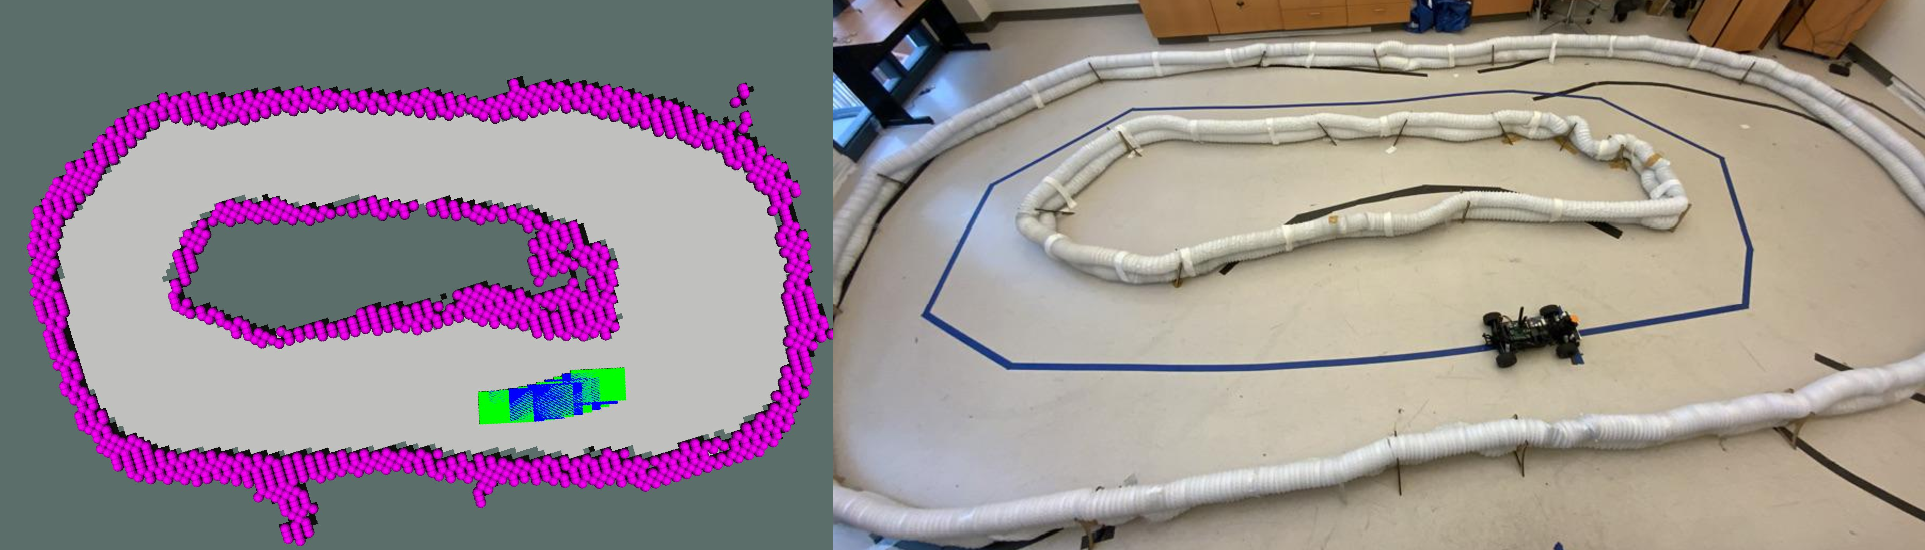
\includegraphics[width=\linewidth]{figures/sidebyside_comparison.pdf}
  \caption{Visualization of the hardware experiments on the F1/10 Platform, the magenta points are the point-discretization of the wall boundaries (not all points are visualized). Videos of the experiments can be found at}
%   \url{https://github.com/pmusau17/F1TenthHardware}.}
  \label{fig:lab_setup}
\end{figure}%

\begin{table}[ht]%
\renewcommand{\arraystretch}{1.3}
\caption{Analysis of Wall-Time and Speed Variation: Jetson TX2}
\label{tab:hardware}
\centering
\resizebox{0.7\linewidth}{!}{
\begin{tabular}{ccccccccc}
ML Controller &   $u$ (m/s) &  $T_{runtime}$ & MOET (ms) &  Mean ET (ms) &  Mean Iters &  ML Usage (\%) & PMD(\%) \\
\hline

VBN & 0.5 & 10 &  10.87 $\pm$   0.36 &    5.07 $\pm$  0.53 &           5.39 $\pm$  0.83 &    11.70 $\pm$  6.90 &                    0.58 $\pm$  0.29 \\
    &     & 25 &  24.42 $\pm$   0.49 &   10.41 $\pm$  0.63 &           7.56 $\pm$  0.97 &    12.38 $\pm$  2.79 &                    0.00 $\pm$  0.00 \\
    & 1.0 & 10 &  14.36 $\pm$   5.74 &    5.56 $\pm$  0.58 &           5.12 $\pm$  0.39 &     9.31 $\pm$  5.07 &                    1.61 $\pm$  1.18 \\
    &     & 25 &  31.60 $\pm$  17.81 &    9.36 $\pm$  0.79 &           8.69 $\pm$  1.16 &     9.97 $\pm$  2.92 &                    0.03 $\pm$  0.06 \\
LBC & 0.5 & 10 &  24.49 $\pm$  17.76 &    5.35 $\pm$  0.45 &           4.65 $\pm$  0.23 &    20.61 $\pm$  7.43 &                    0.78 $\pm$  0.62 \\
    &     & 25 &  31.31 $\pm$  14.46 &    9.65 $\pm$  0.51 &           6.49 $\pm$  0.82 &    24.28 $\pm$  7.63 &                    0.07 $\pm$  0.07 \\
    & 1.0 & 10 &  14.25 $\pm$   1.81 &    5.18 $\pm$  0.36 &           4.50 $\pm$  0.17 &    17.83 $\pm$  4.75 &                    0.75 $\pm$  0.40 \\
    &     & 25 &  24.43 $\pm$   0.59 &    9.35 $\pm$  0.74 &           7.35 $\pm$  1.02 &    14.38 $\pm$  6.18 &                    0.01 $\pm$  0.03 \\
SAC & 0.5 & 10 &  10.98 $\pm$   0.33 &    5.10 $\pm$  0.16 &           4.97 $\pm$  0.54 &    16.44 $\pm$  9.43 &                    1.74 $\pm$  0.80 \\
    &     & 25 &  26.78 $\pm$   2.57 &   10.91 $\pm$  0.78 &           6.06 $\pm$  0.72 &    26.17 $\pm$  8.21 &                    0.07 $\pm$  0.04 \\
    & 1.0 & 10 &  11.46 $\pm$   0.47 &    4.73 $\pm$  0.54 &           5.65 $\pm$  2.17 &    12.58 $\pm$  3.40 &                    0.61 $\pm$  0.18 \\
    &     & 25 &  27.16 $\pm$   6.38 &    9.69 $\pm$  1.17 &           8.10 $\pm$  0.91 &     9.82 $\pm$  3.07 &                    0.06 $\pm$  0.10 \\
ARS & 0.5 & 10 &  13.92 $\pm$   6.32 &    4.94 $\pm$  0.30 &           5.63 $\pm$  0.38 &    15.88 $\pm$  1.78 &                    0.46 $\pm$  0.35 \\
    &     & 25 &  30.83 $\pm$  15.55 &    9.55 $\pm$  0.53 &           7.00 $\pm$  0.66 &    21.17 $\pm$  6.56 &                    0.02 $\pm$  0.04 \\
    & 1.0 & 10 &  11.53 $\pm$   1.22 &    5.32 $\pm$  0.20 &           4.93 $\pm$  0.55 &    19.95 $\pm$  6.65 &                    1.13 $\pm$  1.13 \\
    &     & 25 &  30.58 $\pm$   9.60 &    8.89 $\pm$  0.72 &           7.50 $\pm$  0.76 &    23.58 $\pm$  3.16 &                    0.05 $\pm$  0.05 \\
\end{tabular}}%
% \footnotemark{CC refers to the complex controller, and SC refers to the safe controller. The results displayed in this table were conducted on the Dell Precision 7520.}
\end{table}


We evaluated the proposed safety regime on the F1/10 hardware platform with two minor differences. Firstly, due to the space constraints of our laboratory environment, we did not consider the addition of obstacles within the racetrack. Our experimental setup is shown in \figref{fig:lab_setup}. Secondly, we chose to offload the machine learning components to a separate computer. Compared to the other controllers the VBN required a prohibitively large amount of the computation resources on the Jetson TX2. It is possible to optimize these ML models to run more efficiently on the Jetson platform, but we elected not to do so as our primary concern was to analyze the variation of execution times of our safety regime on the embedded platform. Additionally, offloading the expensive machine learning computations to another computer allowed us to evaluate our regime with a finer level of granularity, providing a fairer comparison of the controllers.








%\ttj{may want to clarify previous a bit more, someone may comment on this set up; I revised a bit, I assume you ran the real-time reachability on the jetson, and the ML models on a desktop, but double check; likewise, may want to give names for these machines to make it clearer what is running where}



% \begin{table}[h]%
% \renewcommand{\arraystretch}{1.3}
% \caption{Analysis of Wall-Time and Speed Variation: Jetson TX2}
% \label{tab:sim3}
% \centering
% \resizebox{0.8\linewidth}{!}{
% \begin{tabular}{cccccccc}
%     ML Controller & $T_{runtime}$ & $u$ (m/s) & Expected ET (ms) & Expected Iters & ML Usage (\%) & SC Usage (\%) & std \\
%     \hline
%  ARS & 0.5 & 10 &   11.24 $\pm$ 0.47 &         9.13 $\pm$ 0.34 &    55.19 &    44.81 &   2.43 \\
%     &     & 25 &   25.71 $\pm$ 1.05 &          10.01 $\pm$ 0.37 &    55.26 &    44.74 &   2.95 \\
%     & 1.0 & 10 &    9.92 $\pm$ 1.71 &          10.65 $\pm$ 1.80 &    26.44 &    73.56 &   3.52 \\
%     &     & 25 &   24.38 $\pm$ 4.26 &          11.38 $\pm$ 1.66 &    26.39 &    73.61 &   3.81 \\
%     & 1.5 & 10 &    9.72 $\pm$ 1.54 &          10.72 $\pm$ 1.63 &    14.39 &    85.61 &   1.89 \\
%     &     & 25 &   22.12 $\pm$ 3.40 &          11.83 $\pm$ 1.54 &    14.11 &    85.89 &   2.04 \\
% \end{tabular}}%
% % \footnotemark{CC refers to the complex controller, and SC refers to the safe controller. The results displayed in this table were conducted on the Dell Precision 7520.}
% \end{table}



We ran a total of 80 experiments, 5 for each controller, with the same structure as the simulation episodes. A video of the experiments is available online.\footnote{\url{https://streamable.com/zo4ocp}} The results of these experiments demonstrated a large increase in the amount of time that the safety controller was used and a corresponding decrease in the execution time of the approach. However, this result can be explained by the size of our racetrack as well as the known challenges of using ML controllers within the real world. Still, there were no collisions observed in the hardware experiments.

Within the real-time reachability algorithm, the reachable-set computations terminate whenever an unsafe state is detected. The algorithm then restarts with half the step-size in order to refine the over-approximation error and determine if the "unsafe" declaration is spurious. This strategy continues until the step size falls below a pre-specified threshold specified to guarantee numerical stability. On the hardware platform, this threshold was met consistently, which demonstrates the frequency of unsafe declarations. Evidence for this observation is provided in Tables~\ref{tab:additional} and \ref{tab:hardware}. Experiments with higher levels of safety utilize fewer iterations in constructing the reachable set and generally have higher execution times. 
The numerical stability termination conditions are discussed in more detail in~\cite{Johnson2016}.







\section{Discussion}

Having evaluated the applicability of our approach and a timing analysis of the real-time reachability algorithm, we now present some observations based on our results with respect to real-time systems and in the light of the proverbial simulation to real-world gap  that arises not only in the safety assurance research literature but also within artificial intelligence at large.

%\subsection{Threat to Real-Time Validity}

%The basic requirement for real-time systems is that tasks operate within pre-defined and deterministic time spans. Often this is accomplished through the use of a real-time operating system (RTOS), which allows for the specification of task priorities so that they are executed within established time frames. Our implementation did not make use of an RTOS, thus task management was left to the native Linux implementation. Our experimental evaluation demonstrated deviations from the specified wall-time but the mean percent of missed deadlines on the Jetson TX2 was fewer than 2\% across all of our experiments. %Our future work will consider the use of an RTOS so that the reachability computation can be prioritized over other foreground and background tasks.

\subsection{More Missed Deadlines in Simulation}

In our hardware experiments, shown in Table \ref{tab:hardware}, the percentage of missed deadlines (PMD) remained consistent when $T_{runtime}$ was increased from $10ms$ to $25ms$. However, in our simulation experiments, shown in Table \ref{tab:additional}, the PMD increases after $T_{runtime}$ is increased. This difference in results was caused by undesirable context switching. 

In our simulation experiments, a single computer is running all of the ROS nodes as well as the simulation software. In order to prevent all of the nodes from missing their publish deadlines, the simulation utilizes a slower simulation time, which is separate from the wall time we use for our reachability method. Using simulation time allows all nodes to meet their publishing deadlines and increases the amount of context switching going on. If computation load is low, each node can finish it's business without being halted. In our simulations, this isn't the case. So, when we increase $T_{runtime}$, there are more chances for the process to be halted for something else to run. This increases the runtime resulting in more missed deadlines.

In our hardware experiments, we combated this issue by limiting the number of tasks running on the Jetson TX2 to only the essential ROS nodes and ran the NN computations on a separate machine to reduce the computational load. Thus we reduce the number of instances our reachability process is halted to quickly run a different node with an immediate publishing deadline. 

In future work, we could further reduce the percentage of missed deadlines by increasing the conservativeness of the estimate or adding a computation resource focused only on the safety decision similar to how we moved the NN computations to a separate machine.

% Our experimental evaluation demonstrated deviations from the specified wall-time but the mean percent of missed deadlines on the Jetson TX2 was fewer than 2\% across all of our experiments.

\subsection{Challenges Moving from Simulation to the Real World}

Moving from simulation to the real-world hardware platform saw a significant expansion in the frequency that the safety controller was used. This increased reliance on the safety controller is a direct result of \emph{sim2real} challenges in machine learning. Because the real world is inherently more noisy and more complex than the simulation environments that machine learning models are typically trained in, when these models are deployed in the real world, they are tasked with making generalizations on data that may significantly differ from their training distribution. Furthermore, this challenge is exacerbated by the reality of imperfect dynamic and sensor perception models \cite{ivanov2020case}.

The challenges that we faced during the transition from simulation to reality arose in two main fashions: the small track size and environment-induced sensor noise.

\subsubsection{The Small Track} The track shown in \figref{fig:reachset} is much larger than the real world track we tested on, shown in \figref{fig:lab_setup}. At the narrowest point, the simulated track is $2m$ wide.\footnote{Races held by the F1/10 community are around typically 30-50 meters in length with a minimum of 3 meters between the racetrack walls. The rules are described in more detail here: \url{https://f1tenth.org/misc-docs/rules.pdf}} In contrast, the widest part of our track is scarcely larger than that. The bulk of the racetrack has a width of less than one meter. Since $T_{runtime}$ is constant across the simulation and real world experiments, the real world vehicle spends the majority of its time forecasting unsafe actions due to its close proximity to the track walls. The hardware experiments were quite revelatory in motivating our desire to extend the current methodologies to integrate closed-loop reachability techniques. Our current assumption that the control decision remains fixed throughout the reachset construction is quite conservative. Closed-loop reachability techniques would allow us to weaken this assumption and compute approximations of the real inputs during the reachset construction. However, the difficulty in performing closed-loop reachset generation lies in developing accurate sensor models. As an example, for the VBN it is not clear how to generate camera images based on the state of the system so as to provide a meaningful and useful reachable set.
%\diego{Maybe mention something along the lines where this F1Tenth idea comes from: F1. Mention that the simulation track looks like how it should look, but due to space constraints we could not replicate this. TRACK SPECIFICATION (F1): Track width– 12 to 15 metre. This avoids bad congestion. There should be 3 m minimum clear space along both sides of the track, usually consisting of grass.}

\subsubsection{Environment-Induced Noise} Noisy sensor data is expected because no sensor is always perfectly accurate. However, environment-induced noise refers to additional noise that exists because of differences in the environments. This is best highlighted in the case of the RL controller. The environment the agent trained in had smooth, solid walls. Meanwhile, our track is made out of a series of flexible vinyl duct piping hose segments\footnote{\url{https://www.amazon.com/dp/B01G198P8W?psc=1}}, which contain ridges and occasionally expose gaps in between the stacked structure.
While it is possible to try and model these variations in the simulator, this was not within the scope of our study. However, our future work will explore the relationship between simulator fidelity and the safety of each controller. Since the controllers are "black box" in nature, we cannot know for sure how the policies will respond to these variations. Despite this challenge, we were able to get the F1/10 vehicle to successfully complete laps in the real world because of our simplex architecture. The overall performance might have been reduced, but we were able to ensure safe operation.

\section{Related Work}

As cyber-physical systems have become increasingly more complex in recent years, there has been a major thrust to develop techniques capable of assuring their safety at at runtime. % There has been a wealth of exciting works that attempt to prove the correctness of these systems prior to fielding them in their respective operational design domains, and a nice summary of these works is contained in the following papers \cite{Maler14,Tomlin2003,Doyen2018,Yang2017,Clark2013,Kwon2018}. In certain environments, however, complete or even partial verification may be infeasible due to the well-known state-explosion problem \cite{Valmari1998}, and the challenge may further be exacerbated by the opaqueness of the components considered. 
This has led to the rise of \textit{simplex}, \textit{runtime assurance}, and \textit{runtime-verification} strategies, and it is within this context that we present our work.


\begin{table}[htbp]
\renewcommand{\arraystretch}{1.3}
\caption{Comparison of Online Reachability and Monitoring Methods %\ttj{if space is an issue, may want to use yes/no instead of true/false (or checkmark/xmark), and may want to make the header row multirow to make layout cleaner, or use an acronym for the header row titles and describe the acronym in this caption; I would add a row for this paper and highlight that in the earlier rtreach it has not been applied to LECs; also, are you sure any of these other approaches have real-time guarantees? are they just doing offline reachability, then monitoring online? may want to have a column for that or highlight that}
}
\label{tab:related_work}
\centering
\resizebox{0.7\linewidth}{!}{
\begin{tabular}{cccccc}
     & Real-Time & External & Evaluation & ML & Online\\
     Tool Name & Guarantee & Libraries  & Platforms & Monitoring& Reachability\\
    \hline
 Rtreach-ML (this paper)& \checkmark & $\times$ & x86,ARM & \checkmark & \checkmark\\
 
 Rtreach \cite{Johnson2016} &  \checkmark & $\times$ & x86, ARM, AVR & $\times$ & \checkmark\\
 
 BACH2 \cite{Bu2011,BU2020} & $\checkmark$ & \checkmark & x86     & $\times$ & \checkmark\\
 
 ReachFlow (Flow*) \cite{Lin2020}  & $\times$ & \checkmark & x86     & \checkmark & \checkmark \\
 
PHaVer \cite{Ti2014} & $\times$ & \checkmark & x86     & $\times$ & \checkmark \\
FaSTrack \cite{HerbertFastrack} & $\times$ & \checkmark & x86    & $\times$ & $\times$ \\

 ARMTD \cite{holmes2020reachable} & $\checkmark$  & \checkmark & x86  & $\times$ & $\times$ \\
 
CORA \cite{Althoff2014} & $\checkmark$  & \checkmark & x86  & $\times$ & $\checkmark$ \\
  
SafeTrafficWeaving \cite{LeungReach2020} & $\checkmark$ & \checkmark & x86  & $\times$ & $\times$  \\
  
ROSRV \cite{Huang2014} & $\times$ & \checkmark & x86  & $\times$ & $\times$ \\
   
SOTER \cite{Desai2018,Desai2017} & $\times$ & \checkmark & x86  & $\times$ & $\times$ \\
    
Modelplex/VeriPhy \cite{mitsch} & $\times$ & \checkmark & x86, ARM  & $\times$ & $\times$ \\

Black-Box Simplex \cite{Mehmood2021}  & $\times$ & \checkmark & x86 & $\checkmark$ & $\checkmark$ \\

FPGA HJR \cite{Bui2021} & $\checkmark$ & \checkmark & x86, ARM & $\times$ & $\times$ \\


    % \vspace{0.1cm}
\end{tabular}}
% \footnotemark{CC refers to the complex controller, and SC refers to the safe controller.}
\end{table}%
%\diego{I have some questions about this table... Why is CORA there? In the paper they mention they do online reachability but they table says they do not. They also mention that their code is in C++ but CORA is written in MATLAB, and based on the quick glance I took at it, I'm unsure those methods are implemented in CORA, but I have not really checked.}


The simplex architecture has been used widely in the research literature to provide guarantees for systems with unverified logic. The contexts in which it has been applied include aerospace systems \cite{SetoCaseStudy2000}, fleets of remote controlled cars \cite{Crenshaw2007}, industrial embedded infrastructure \cite{Bak2009Simplex,Yang2017}, and distributed mobile robotics applications \cite{Desai2018,Tran2020}. In \cite{Lin2020}, the authors utilize a reachability regime to guarantee the safety of an autonomous vehicle that makes use of a reinforcement learning controller for a way-point-following task. Most similar to this work in \cite{Tran2020}, the authors utilize a real-time reachability approach to verify that a group of quadcopters executing a distributed search mission defined by a series of waypoints is free from collisions. Their approach is implemented in simulation and can theoretically deal with over 64 quadcopters. These works primarily deal with developing provably correct motion planners, while the focus of this work is abstracting away the underlying nature of a set of ML components and reasoning about the consequence of their actions on overall system safety.



%In \cite{Desai2018}, Desai et al. propose an architecture for building reliable distributed mobile robotics by using a state-machine based language for safe event-driven programming. Like this work, their solution can be deployed within ROS, and the authors assume a known environment with static obstacles. However, their work is primarily focused on developing a provably correct motion planner, while this work projects the consequences of the control actions issued by a controller. In a similar work by Huang et al. \cite{Huang2014}, the authors present a run-time verification framework named ROSRV, which provides a specification language for ensuring safety and security properties within robotic applications. It allows for properties that can be expressed using temporal logic and regular expressions, and their techniques were demonstrated on a unmanned ground vehicle.

Closely related to simplex techniques are runtime assurance (RTA) methods and runtime verification (RV) methods. An intuitive explanation of these regimes can be summarized as follows. RTA techniques are tasked with ensuring the safe operation of systems with untrusted components, while runtime verification techniques monitor a system against presupposed formal properties at runtime 
%\cite{PETTERSSON200573,DesaiRV2017,Deshmukh2015,Masson2018,Akametalu2014,mitsch,Daws1998,Phan2020}. 
\cite{Masson2018,Akametalu2014,mitsch,Daws1998,Phan2020}. The distinction here is that while runtime assurance techniques may often utilize verification results, they may often also employ statistical techniques such as anomaly detection \cite{boursinos2020trusted} or simulation based strategies \cite{TranSimulation2019}. %One such example is the work by Allen et al.\cite{Allen2014}, in which they utilize various machine learning techniques, mainly support vector machines and linear regression models, to approximate the solution to the real-time reachability problem. Their work is capable of being applied in low-resource, real-time environments but suffers from the downside that theoretical guarantees cannot be made using these techniques, only statistical ones. However, it demonstrated impressive results in improving state-of-the-art execution times by four orders of magnitude.

Finally, in recent years, researchers have begun to integrate traditionally non real-time approaches within real-time systems, making these approaches more amenable to real-time execution. These include viability kernel approaches that determine if a set of states remain within a predefined region \cite{Gurriet2018,Althoff2014}, as well as Hamilton-Jacobi reachability (HJR) techniques that deal with dynamical systems with general nonlinear dynamics and disturbances in uncertain environments \cite{Herbert2019,Bajcsy2019Provably,bansal2020hamiltonjacobi,Fisac2017,Chen2016,dhinakaran2017hybrid}. Specifically, \cite{Bajcsy2019Provably} and \cite{Althoff2014} were able to implement their techniques both in simulation and on hardware platforms. However, both papers used their respective real-time reachability results for safe real-time motion planning, while the work contained in this paper primarily dealt with the construction and implementation of the simplex architecture. 

%In a similar vein, in \cite{LeungReach2020} Leung et al. proposed a safety-assurance control architecture based on HJI reachability for traffic weaving experiments. Their approach uses both forward and backward reachability techniques in order to integrate safety constraints into a model predictive controller tasked with trajectory generation. Their approach differs from this work in that they seek to minimize the intervention of safety control actions to situations where they are strictly required. 


Table \ref{tab:related_work} presents several state-of-the-art online reachability tools present within the literature and summarizes their amenability to real-time operation. What distinguishes the methods presented in this work is that they possess real-time guarantees and have been extended from \cite{Johnson2016} for the monitoring of machine learning models. Particularly, our work is to the best of our knowledge the only work that deals with perception controllers. We realize that there are numerous other interesting works present within this area, and to the best of our knowledge, the aforementioned works are the most relevant to the methods presented within this paper.   

\section{Conclusions and Future Work}

In this work we proposed a simplex architecture for the safety assurance of a one-tenth scale autonomous car through the use of a real-time reachability algorithm compatible with the anytime computation model in the real-time scheduling literature. Our experiments conducted both in simulation and on an open-source embedded hardware platform validate the real-time aspects of our approach and demonstrate its efficacy in assuring safety in different scenarios. Furthermore, we have presented a method for providing formal guarantees for a variety of controllers by abstracting away the need to formally analyze these controllers and instead reason online about the the future effect of their decisions on system behavior through the use of reachability analysis. Improving the over-conservativeness of the reachability framework,  closed-loop reach-set generation, and incorporating dynamic obstacles into our regime are left for future work.


%\diego{What does it mean to validate real time aspects? Where is this done?}

%In the future, we hope to expand the work shown in this manuscript to include closed-loop reachability analysis. The current approach is limited to repeating the same control action for the duration of the reach time. This assumption results in an overly conservative use of the safety controller. %, which could prevent mission critical tasks from being performed in certain contexts. 
%We did not consider closed-loop reach-set generation within our context due to the difficulties in developing an accurate sensor model. More specifically, it is not clear how to generate synthetic camera images that would provide a meaningful and useful reachable set. Even when the only sensor considered is the lidar, constructing an accurate sensor model is quite complicated, as shown by Ivanov et al. \cite{ivanov2020case}. In the future, we hope to work toward developing useful sensor models through the use of Generative Adversarial Networks, which are known for their ability to synthesize new examples that plausibly come from an existing distribution of samples \cite{Radford2016,Brock2018,goodfellow2014}. \diego{Really? GANs with ever-growing reach sets (position, angle...) But then at that point is not really close-loop reachability, but a more probable/better prediction of controller's output at next steps...}

%\todo{Take a look at the references, some of them aren't displaying author's properly...}

\bibliographystyle{acm}
\bibliography{references.bib}


\appendix
%\section{Additional Experiments}
%\label{app:experiments}






\end{document}
\endinput